% arara: xelatex
% arara: biber
% arara: xelatex: { synctex: true }

\documentclass[12pt,a4paper,oneside,final]{report}

\usepackage{tabularx}
\usepackage{booktabs}

\usepackage{polyglossia}
\setmainlanguage[numerals=cyrillic]{russian}
\setotherlanguages{english}
\usepackage{csquotes}

% \usepackage{xunicode} % some extra unicode support
%\usepackage[utf8x]{inputenc}
\usepackage{xltxtra} % \XeLaTeX macro
\usepackage{fontspec}
\defaultfontfeatures{Ligatures=TeX}

%\setromanfont{Charis SIL}
%\setsansfont{Liberation Sans}
%\setmonofont{PT Mono}
%\setmainfont{Liberation Serif} % this allows to use sans-serif as default font


\newfontfamily\cyrillicfont{Times New Roman}
\newfontfamily\cyrillicfontsf{Arial}
\newfontfamily\cyrillicfonttt{Courier New}

\setmainfont{Times New Roman}
\setsansfont{Arial}
\setmonofont{Courier New}

\newfontfamily\englishfont[Script=Latin, Contextuals={WordInitial,WordFinal}]{Times New Roman}
\setotherlanguage[Numerals=Latin]{english}

%нумерация справа и колонтитулы справа вверху
\usepackage{fancyhdr}
\usepackage[a4paper,left=30mm,right=15mm,top=20mm,bottom=20mm,bindingoffset=0cm]{geometry}%

\usepackage{amsfonts}
\usepackage{amssymb}
\usepackage{amsmath}
\usepackage{amsthm}

\usepackage{calc}
\usepackage{ifthen}
\usepackage{graphicx}
\usepackage{array}
\usepackage{pdfpages}
\usepackage{longtable}
\usepackage{multirow}
\usepackage{indentfirst}
\usepackage[unicode=true]{hyperref}
\usepackage{color}
\usepackage{pgf}
\usepackage{1-preamble/pstheorems}
\usepackage{titling}

% Настройка списков (без лишних вертикальных отступов)
\usepackage{paralist}
\setdefaultenum{1.}{1.}{1.}{1.}
\setdefaultitem{--}{}{}{}
%\setlength\itemsep{-1em}
\let\itemize\compactitem
\let\enditemize\endcompactitem
\let\enumerate\compactenum
\let\endenumerate\endcompactenum
\let\description\compactdesc
\let\enddescription\endcompactdesc
\pltopsep=\smallskipamount
\plitemsep=0pt
\plparsep=0pt
% Команда для отмены разрыва страниц перед списками
\makeatletter
\newcommand\mynobreakpar{\par\nobreak\@afterheading}
\makeatother
%%%%%%

\usepackage[singlelinecheck=false,labelsep=endash]{caption}
\captionsetup[table]{justification=justified}
\captionsetup[figure]{justification=justified,name=Рисунок,singlelinecheck=on,font=onehalfspacing}

\usepackage{titlesec}
\titleformat{\chapter}[block]{\centering\normalfont\Large\bfseries}{\thechapter.}{1ex}{}{}
\titlespacing{\chapter}{0pt}{0em}{2em}

\titleformat{\section}[block]{\normalfont\large\bfseries}{\thesection}{1ex}{}{}
\titlespacing{\section}{0pt}{0em}{1ex}

\titleformat{\subsection}[block]{\normalfont\normalsize\bfseries}{\thesubsection}{1ex}{}{}
\titlespacing{\section}{0pt}{0em}{1ex}

% paragraph и subparagraph -- в тексте, без отступов
\titleformat{\paragraph}[runin]{\normalfont\normalsize\bfseries}{\theparagraph}{0pt}{}{}
\titlespacing{\paragraph}{0pt}{0em}{0ex}

\titleformat{\subparagraph}[runin]{\normalfont\normalsize\bfseries}{\thesubparagraph}{0pt}{}{}
\titlespacing{\subparagraph}{0pt}{0em}{0ex}


% Своё название для Cписка литературы
\usepackage[title, titletoc]{appendix}
\addto\captionsrussian{% Replace "english" with the language you use
  \renewcommand{\contentsname}%
  {Содержание}%
}

%\renewcommand{\appendixname}{Приложение}% Change "chapter name" for Appendix chapters
%\renewcommand{\cftchapdotsep}{\cftdotsep}

\usepackage{mathpartir}

\makeatletter
\let\ps@plain\ps@fancy              % Подчиняем первые страницы каждой главы общим правилам
\makeatother
\pagestyle{fancy}
\fancyhf{}
\fancyfoot[C]{\thepage}
\renewcommand{\headrulewidth}{0pt}
\renewcommand{\footrulewidth}{0pt}
\renewcommand{\baselinestretch}{1.5}
\newcommand{\headertext}[1]{\fancyhead[R]{\tiny{#1}}}

%% Список литературы

\usepackage[
  style=gost-numeric,
  sorting=none,
  language=auto,
  autolang=other
]{biblatex}
\addbibresource{5-bibliography/bibliography.bib}

\usepackage{tikz}
\usepackage{hhline}

\graphicspath{{assets/img}}

%\frenchspacing %% изменение расстояние до и после точек в ряде случаев

\renewcommand{\theenumi}{\arabic{enumi}}
\renewcommand{\theenumii}{\arabic{enumii}}
\renewcommand{\theenumiii}{\arabic{enumiii}}
\renewcommand{\theenumiv}{\arabic{enumiv}}

\renewcommand{\labelenumi}{\theenumi.}
\renewcommand{\labelenumii}{\theenumi.\theenumii.}
\renewcommand{\labelenumiii}{\theenumi.\theenumii.\theenumiii.}
\renewcommand{\labelenumiv}{\theenumi.\theenumii.\theenumiii.\theenumiv.}

%\newenvironment{annotation}{\textbf{Аннотация.} \textit}{}
\theoremstyle{plain}
\newtheorem*{annotation}{Аннотация}

\makeatletter
\newcommand*{\projecttypefulldative}[1]{\gdef\@projecttypefulldative{#1}}
\newcommand*{\theprojecttypefulldative}{\@projecttypefulldative}
\newcommand*{\projecttypeshort}[1]{\gdef\@projecttypeshort{#1}}
\newcommand*{\theprojecttypeshort}{\@projecttypeshort}
\newcommand*{\authorfulldative}[1]{\gdef\@authorfulldative{#1}}
\newcommand*{\theauthorfulldative}{\@authorfulldative}
\newcommand*{\authorgroup}[1]{\gdef\@authorgroup{#1}}
\newcommand*{\theauthorgroup}{\@authorgroup}
\newcommand*{\supervisor}[1]{\gdef\@supervisor{#1}}
\newcommand*{\thesupervisor}{\@supervisor}
\newcommand*{\consultant}[1]{\gdef\@consultant{#1}}
\newcommand*{\theconsultant}{\@consultant}
\newcommand{\projecttasks}[1]{\gdef\@projecttasks{#1}}
\newcommand{\theprojecttasks}{\@projecttasks}
\newcommand{\projecttask}[5]{#1 & #2 & #3 & #4 & #5 \\\hline}
\newcommand*{\taskliterature}[1]{\gdef\@taskliterature{#1}}
\newcommand*{\thetaskliterature}{\@taskliterature}
\newcommand*{\taskdate}[1]{\gdef\@taskdate{#1}}
\newcommand*{\thetaskdate}{\@taskdate}
\newcommand*{\supervisortaskapproval}[1]{\gdef\@supervisortaskapproval{#1}}
\newcommand*{\thesupervisortaskapproval}{\@supervisortaskapproval}
\newcommand*{\authortaskapproval}[1]{\gdef\@authortaskapproval{#1}}
\newcommand*{\theauthortaskapproval}{\@authortaskapproval}
\newcommand*{\authorrspzapproval}[1]{\gdef\@authorrspzapproval{#1}}
\newcommand*{\theauthorrspzapproval}{\@authorrspzapproval}
\newcommand*{\supervisorrspzapproval}[1]{\gdef\@supervisorrspzapproval{#1}}
\newcommand*{\thesupervisorrspzapproval}{\@supervisorrspzapproval}
\newcommand*{\consultantrspzapproval}[1]{\gdef\@consultantrspzapproval{#1}}
\newcommand*{\theconsultantrspzapproval}{\@consultantrspzapproval}
\newcommand*{\supervisorrspzgrade}[1]{\gdef\@supervisorrspzgrade{#1}}
\newcommand*{\thesupervisorrspzgrade}{\@supervisorrspzgrade}
\newcommand*{\consultantrspzgrade}[1]{\gdef\@consultantrspzgrade{#1}}
\newcommand*{\theconsultantrspzgrade}{\@consultantrspzgrade}
\newcommand*{\authorpzapproval}[1]{\gdef\@authorpzapproval{#1}}
\newcommand*{\theauthorpzapproval}{\@authorpzapproval}
\newcommand*{\supervisorpzapproval}[1]{\gdef\@supervisorpzapproval{#1}}
\newcommand*{\thesupervisorpzapproval}{\@supervisorpzapproval}
\newcommand*{\consultantpzapproval}[1]{\gdef\@consultantpzapproval{#1}}
\newcommand*{\theconsultantpzapproval}{\@consultantpzapproval}
\newcommand*{\supervisorpzgrade}[1]{\gdef\@supervisorpzgrade{#1}}
\newcommand*{\thesupervisorpzgrade}{\@supervisorpzgrade}
\newcommand*{\consultantpzgrade}[1]{\gdef\@consultantpzgrade{#1}}
\newcommand*{\theconsultantpzgrade}{\@consultantpzgrade}
\makeatother

%% Настройка подписей
\makeatletter
\pgfkeys{
  /signat/.is family, /signat,
  xsign/.initial=-10pt,
  ysign/.initial=4pt,
  scale/.initial=0.3,
  img/.initial=supervisor,
  xdate/.initial=10pt,
  ydate/.initial=-10pt,
  date/.initial=01.01.2001
}
\makeatother

% Разные подписи для локального и публичного репозиториев
\IfFileExists{3-content/00-project-members-local}{
  % ==== LOCAL ====
  \newcommand{\signaturepath}{assets/signatures/local/}
  \newcommand{\sign}[3][0pt]{%
    \tikz[overlay]{\node[yshift=##1]{\includegraphics[scale=##2]{\signaturepath##3.png}}}%
  }
  \NewDocumentCommand{\signat}{O{}}{%
    \pgfkeys{/signat, ##1}%
    \begin{tikzpicture}[overlay]
      \node[xshift=\pgfkeysvalueof{/signat/xsign}, yshift=\pgfkeysvalueof{/signat/ysign}](c)
      {\includegraphics[scale=\pgfkeysvalueof{/signat/scale}]{\signaturepath\pgfkeysvalueof{/signat/img}.png}};
      \node[xshift=\pgfkeysvalueof{/signat/xdate}, yshift=\pgfkeysvalueof{/signat/ydate}]
      {\small\textit{\pgfkeysvalueof{/signat/date}}};
    \end{tikzpicture}
  }
}{
  % ==== PUBLIC ====
  \newcommand{\signaturepath}{assets/signatures/public/}
  \newcommand{\sign}[3][0pt]{%
    % Аргументы игнорируются, фиксированная заглушка
    \tikz[overlay]{\node[yshift=10pt]{\includegraphics[scale=.15]{\signaturepath##3.png}}}%
  }
  \NewDocumentCommand{\signat}{O{}}{%
    \pgfkeys{/signat, ##1}%
    \begin{tikzpicture}[overlay]
      \node[xshift=-15pt, yshift=7pt](c)
      {\includegraphics[scale=0.1]{\signaturepath\pgfkeysvalueof{/signat/img}.png}};
      \node[xshift=15pt, yshift=-2pt]
      {\small\textit{\pgfkeysvalueof{/signat/date}}};
    \end{tikzpicture}
  }
}

\newcommand{\emptyfield}{\tikz[overlay]{\draw[thin,yshift=-1.28ex](0,0)--(5,0)}}

\newcounter{projecttasknumber}
\newcommand{\projecttasknum}{\setcounter{projectsubtasknumber}{0}\stepcounter{projecttasknumber}\theprojecttasknumber.}

\newcounter{projectsubtasknumber}
\newcommand{\projectsubtasknum}{\stepcounter{projectsubtasknumber}\theprojecttasknumber.\theprojectsubtasknumber.}

\usepackage{listings}

\renewcommand{\lstlistingname}{Листинг}

\lstset{
basicstyle=\linespread{0.94}\ttfamily\small,
tabsize=2,
showstringspaces=false,
columns=flexible,
numbers=none,
numberstyle=\tiny\color{gray},
breaklines=true,
breakatwhitespace=true,
framesep=6pt,
abovecaptionskip=1em,
captionpos=t,
extendedchars=true,
inputencoding=utf8,
literate={Ö}{{\"O}}1
{Ä}{{\"A}}1
{Ü}{{\"U}}1
{ß}{{\ss}}1
{ü}{{\"u}}1
{ä}{{\"a}}1
{ö}{{\"o}}1
{~}{{\textasciitilde}}1
{а}{{\selectfont\char224}}1
{б}{{\selectfont\char225}}1
{в}{{\selectfont\char226}}1
{г}{{\selectfont\char227}}1
{д}{{\selectfont\char228}}1
{е}{{\selectfont\char229}}1
{ё}{{\"e}}1
{ж}{{\selectfont\char230}}1
{з}{{\selectfont\char231}}1
{и}{{\selectfont\char232}}1
{й}{{\selectfont\char233}}1
{к}{{\selectfont\char234}}1
{л}{{\selectfont\char235}}1
{м}{{\selectfont\char236}}1
{н}{{\selectfont\char237}}1
{о}{{\selectfont\char238}}1
{п}{{\selectfont\char239}}1
{р}{{\selectfont\char240}}1
{с}{{\selectfont\char241}}1
{т}{{\selectfont\char242}}1
{у}{{\selectfont\char243}}1
{ф}{{\selectfont\char244}}1
{х}{{\selectfont\char245}}1
{ц}{{\selectfont\char246}}1
{ч}{{\selectfont\char247}}1
{ш}{{\selectfont\char248}}1
{щ}{{\selectfont\char249}}1
{ъ}{{\selectfont\char250}}1
{ы}{{\selectfont\char251}}1
{ь}{{\selectfont\char252}}1
{э}{{\selectfont\char253}}1
{ю}{{\selectfont\char254}}1
{я}{{\selectfont\char255}}1
{А}{{\selectfont\char192}}1
{Б}{{\selectfont\char193}}1
{В}{{\selectfont\char194}}1
{Г}{{\selectfont\char195}}1
{Д}{{\selectfont\char196}}1
{Е}{{\selectfont\char197}}1
{Ё}{{\"E}}1
{Ж}{{\selectfont\char198}}1
{З}{{\selectfont\char199}}1
{И}{{\selectfont\char200}}1
{Й}{{\selectfont\char201}}1
{К}{{\selectfont\char202}}1
{Л}{{\selectfont\char203}}1
{М}{{\selectfont\char204}}1
{Н}{{\selectfont\char205}}1
{О}{{\selectfont\char206}}1
{П}{{\selectfont\char207}}1
{Р}{{\selectfont\char208}}1
{С}{{\selectfont\char209}}1
{Т}{{\selectfont\char210}}1
{У}{{\selectfont\char211}}1
{Ф}{{\selectfont\char212}}1
{Х}{{\selectfont\char213}}1
{Ц}{{\selectfont\char214}}1
{Ч}{{\selectfont\char215}}1
{Ш}{{\selectfont\char216}}1
{Щ}{{\selectfont\char217}}1
{Ъ}{{\selectfont\char218}}1
{Ы}{{\selectfont\char219}}1
{Ь}{{\selectfont\char220}}1
{Э}{{\selectfont\char221}}1
{Ю}{{\selectfont\char222}}1
{Я}{{\selectfont\char223}}1
{…}{\ldots}1
{–}{-}1
{\ }{ }1
}

\headertext{}


% Условие для того, чтобы имена авторов были вымышленные в публичном репозитории автоматически
\IfFileExists{3-content/00-project-members-local}{
  \input{3-content/00-project-members-local}
}{
  \authorgroup{Б22-555}
\author{Петечкин В. П.}
\authorfulldative{Петечкину Василию Петровичу}
\supervisor{Манилов А. В.}
\consultant{\emptyfield}
\projecttypefulldative{учебно-исследовательской работе}
\projecttypeshort{УИР}
}

\title{Разработка веб-сервиса для запросов к базам данных \\ на естественном языке}

\taskdate{24.02.2025}

\projecttasks{
  \projecttask{\bfseries\projecttasknum}{\bfseries Аналитическая часть}{}{}{}
  % (указываются предмет и цели анализа)
  % ----------------------------------------
  \projecttask{\projectsubtasknum}
  {
    Провести анализ существующих веб-
    сервисов, позволяющих производить запросы
    к базам данных на естественном языке.
  }%
  {Список литературы, текст РСПЗ}%
  {14.03.2025}
  {
    % \signat[xsign=0pt, ysign=-10pt, scale=0.4, xdate=14pt, ydate=-22pt, date={01.01.2001}]
  }
  % ----------------------------------------
  \projecttask{\projectsubtasknum}
  {
    Провести анализ существующих моделей,
    переводящих естественный язык на язык
    запросов SQL.
  }%
  {Список литературы, текст РСПЗ}%
  {24.03.2025}
  {
    % \signat[xsign=-7pt, ysign=-7pt, scale=0.32, xdate=12pt, ydate=-17pt, date={01.01.2001}]
  }
  % ----------------------------------------
  \projecttask{\projectsubtasknum}
  {\itshape
    Оформить расширенное содержание
    пояснительной записки (РСПЗ)
  }%
  {Текст РСПЗ}%
  {28.03.2025}
  {
    % \signat[xsign=-12pt, ysign=-4pt, scale=0.25, xdate=14pt, ydate=-10pt, date={\footnotesize01.01.2001}]
  }
  % ----------------------------------------
  % ----------------------------------------
  \projecttask{\bfseries\projecttasknum}{\bfseries Теоретическая часть}{}{}{}
  % (указываются используемые и разрабатываемые модели, методы, алгоритмы)
  \projecttask{\projectsubtasknum}
  {
    Постановить задачу о проектировании
    внутренней базы данных и разработке блока
    предобработки запросов
  }%
  {Текст ПЗ}%
  {03.04.2025}
  {
    % \signat[xsign=-12pt, ysign=-4pt, scale=0.25, xdate=14pt, ydate=-10pt, date={\footnotesize01.01.2001}]
  }
  % ----------------------------------------
  \projecttask{\projectsubtasknum}
  {Спроектировать внутреннюю базу данных}%
  {Описание моделей БД, текст ПЗ}%
  {10.04.2025}
  {
    % \signat[xsign=-7pt, ysign=-7pt, scale=0.32, xdate=12pt, ydate=-17pt, date={01.01.2001}]
  }
  % ----------------------------------------
  \projecttask{\projectsubtasknum}
  {Разработать блок предобработки запросов}%
  {Текст ПЗ}%
  {17.04.2025}
  {
    % \signat[xsign=-17pt, ysign=-2pt, scale=0.20, xdate=19pt, ydate=0pt, date={\scriptsize01.01.2001}]
  }
  % ----------------------------------------
  % ----------------------------------------
  \projecttask{\bfseries\projecttasknum}{\bfseries Инженерная часть}{}{}{}
  % (указывается, что конкретно необходимо спроектировать, а также используемые для этого методы, технологии и инструментальные средства)
  \projecttask{\projectsubtasknum}
  {
    Установить требования к системе и
    интерфейсу пользователя
  }%
  {Текст ПЗ}%
  {24.04.2025}
  {
    % \signat[xsign=-10pt, ysign=-4pt, scale=0.25, xdate=16pt, ydate=-10pt,
    date={\footnotesize01.01.2001}]
  }
  \projecttask{\projectsubtasknum}
  {Разработать архитектуру веб-сервиса}%
  {Текст ПЗ}%
  {27.04.2025}
  {\
    % % \signat[xsign=-10pt, ysign=4pt, scale=0.25, xdate=17pt, ydate=-2pt, date={\scriptsize01.01.2001}]
  }
  % ----------------------------------------
  \projecttask{\projectsubtasknum}
  {
    Выбрать стек технологий и
    описать причину его выбора
  }%
  {Текст ПЗ}%
  {01.05.2025}
  {
    % \signat[xsign=-12pt, ysign=-4pt, scale=0.25, xdate=14pt, ydate=-10pt, date={\footnotesize01.01.2001}]
  }
  % ----------------------------------------
  \projecttask{\projectsubtasknum}
  {Описать функционал веб-сервиса}%
  {Текст ПЗ}%
  {08.05.2025}
  {
    % % \signat[xsign=-10pt, ysign=4pt, scale=0.25, xdate=17pt, ydate=-2pt, date={\scriptsize01.01.2001}]
  }
  % ----------------------------------------
  \projecttask{\projectsubtasknum}
  {
    Описать программную реализацию системы
    (основные классы и функции)
  }%
  {Текст ПЗ}%
  {17.05.2025}
  {
    % \signat[xsign=-12pt, ysign=-4pt, scale=0.25, xdate=14pt, ydate=-10pt, date={\footnotesize01.01.2001}]
  }
  % ----------------------------------------
  % ----------------------------------------
  \projecttask{\bfseries\projecttasknum}{\bfseries Технологическая и практическая часть}{}{}{}
  % (указывается, что конкретно должно быть реализовано и протестировано, а также используемые для этого методы, инструментальные средства, технологии)
  \projecttask{\projectsubtasknum}
  {
    Протестировать систему на тренировочной
    базе данных
  }%
  {Исполняемые тестовые файлы, текст ПЗ}%
  {19.05.2025}
  {
    % \signat[xsign=-7pt, ysign=-7pt, scale=0.32, xdate=12pt, ydate=-17pt, date={01.01.2001}]
  }
  % ----------------------------------------
  \projecttask{\projectsubtasknum}
  {Описать процесс работы пользователя с веб-сервисом}%
  {Текст ПЗ}%
  {21.05.2025}
  {
    % % \signat[xsign=0pt, ysign=-5pt, scale=0.4, ydate=-20pt, date={\small01.01.2001}]
  }
  % ----------------------------------------
  \projecttask{\bfseries\projecttasknum}
  {\itshape
    Оформить пояснительную записку (ПЗ) и
    иллюстративный материал для доклада
  }%
  {Текст ПЗ, презентация}%
  {22.05.2025}
  {
    % \signat[xsign=-12pt, ysign=-4pt, scale=0.25, xdate=14pt, ydate=-10pt, date={\footnotesize01.01.2001}]
  }
  % ----------------------------------------
  % ----------------------------------------
}

\taskliterature{
  \nocite{
    sidorovEstestvennyeIskusstvennyeYazyki2024,
    kimNaturalLanguageSQL2020,
    borodinZadacheSostavleniyaZaprosov2016,
    polonskiyPerevodRusskogoEstestvennogo2023,
    LLMyPreobrazovaniiZaprosa2023,
    zhuAutomatedCrossdomainExploratory2024
  }
}

% # Подписи

% Для простановки подписи используются слдеющие команды:
% - простая подпись: \sign[<сдвиг>]{<масштаб>}{<FIO>}
% где 
% - <сдвиг> --- необязательный сдвиг подписи по вертикали для правильного
%   расположения относительно строки
% - <масштаб> --- число, используемое для масштарибования изображения подписи
% - <FIO> --- имя файла с подписью, файл должен быть помещен в
%   img/signatures/FIO.png и иметь прозрачный фон
% - <дата> --- дата, которая будет выведена под подписью
%
% - подпись с датой: \signat[xsign=, ysign=, scale=, img=, xdate=, ydate=, date=]
% где все аргументы необязательны и имеют дефолтные значения:
% - xsign(=-10pt) --- сдвиг картинки подписи по горизонтали
% - ysign(=-4pt) --- сдвиг картинки подписи по вертикали
% - scale(=0.3) --- число, используемое для масштарибования изображения подписи
% - img(=supervisor) --- название изображения подписи в папке local или public
% - xdate(=10pt) --- сдвиг даты по горизонтали
% - ydate(=-10pt) --- сдвиг даты по вертикали
% - date(=01.01.2001) --- дата


% ## Утверждение задания руководителем и студентом
\authortaskapproval{\sign[5pt]{.15}{author}}
\supervisortaskapproval{\sign[0pt]{.35}{supervisor}}

% ## Утверждение РСПЗ руководителем, студентом и консультантом
\authorrspzapproval{\sign[10pt]{.20}{author}}
\supervisorrspzapproval{\sign[0pt]{.35}{supervisor}}
\consultantrspzapproval{}

% ## Оценка руководителя и консультанта за РСПЗ
\supervisorrspzgrade{10 б.}
\consultantrspzgrade{}

% ## Утверждение ПЗ руководителем, студентом и консультантом
\authorpzapproval{\sign[10pt]{.20}{author}}
\supervisorpzapproval{\sign[0pt]{.35}{supervisor}}
\consultantpzapproval{}

% ## Оценка руководителя за ПЗ
\supervisorpzgrade{12 б.}
\consultantpzgrade{}


\newcounter{totalfigures}
\newcounter{totaltables}
\newcounter{totallistings}


% В ПЗ мы аннотации выключаются
\showannotationsfalse

\addto{\captionsrussian}{\renewcommand{\bibname}{Список литературы}}

\begin{document}

% Для титульного листа, сверстанного в LaTeX
\thispagestyle{empty}
\begin{center}
  {\scriptsize
    \uppercase{Министерство науки и высшего образования российской федерации}\linebreak
    \uppercase{Федеральное государственное автономное образовательное
      учреждение высшего образования}
  }

  \textbf{Национальный исследовательский ядерный университет «МИФИ»}

  {\footnotesize
    \noindent\makebox[\linewidth]{\rule{\linewidth}{0.4pt}}
  }
\end{center}

\vskip 1em

\noindent
\begin{tabular}{@{}lc@{}}
  \multirow{2}{*}{
\includegraphics[width=0.2\linewidth]{assets/title/mephi.png}}
   & \textbf{\large{}Институт интеллектуальных кибернетических систем} \\
   & \uppercase{\textbf{\large{}Кафедра кибернетики (№ 22)}}           \\
\end{tabular}


\vfill

\begin{center}
  Направление подготовки 09.03.04 Программная инженерия

  \vfill

  {\Large{\textbf{Пояснительная записка}}}

  к \theprojecttypefulldative\space студента на тему:

  {\Large\thetitle}
\end{center}

\vfill

{\large

  \noindent
  \begin{tabularx}{\linewidth}{@{}l>{\centering}XlX@{}}
    Группа              & \raggedright\theauthorgroup &                & \\
    Студент             & \theauthorpzapproval        & \theauthor     & \\ \hhline{~-~}
    Руководитель        & \thesupervisorpzapproval    & \thesupervisor & \\ \hhline{~-~}
    Научный консультант & \theconsultantpzapproval    & \theconsultant & \\ \hhline{~-~}
  \end{tabularx}

  \vfill

  \noindent
  \begin{tabularx}{\linewidth}{@{}cX<{\centering}cX<{\centering}@{}}
    Оценка руководителя & \thesupervisorpzgrade & Оценка консультанта & \theconsultantpzgrade \\ \hhline{~-~-}
    Итоговая оценка     &                       & ECTS                &                       \\ \hhline{~-~-}
  \end{tabularx}

  \vfill

  \center{Комиссия}
  \vspace{1em}
  
  \noindent
  \begin{tabularx}{\linewidth}{@{}lXX@{}}
    Председатель & \emptyfield & \emptyfield \\
                 & \emptyfield & \emptyfield \\
                 & \emptyfield & \emptyfield \\
                 & \emptyfield & \emptyfield \\
  \end{tabularx}

  \vfill

  \begin{center}
    \textbf{Москва \the\year}
  \end{center}

}

\newpage

% Для вставки бланка титульного листа из PDF-файла
% \includepdf[pages={-}, offset=0mm -0mm]{2-titles/title.pdf}

%\clearpage
%% Тут включается лист с подписями для ВКР
%\includepdf[pages={-}, offset=0mm -0mm]{3-titles/title-dep22.pdf}
%\clearpage

% Для листа задания, сверстанного в LaTeX
\pagestyle{empty}
\begin{center}
  {\scriptsize
    \uppercase{Министерство науки и высшего образования российской федерации}\linebreak
    \uppercase{Федеральное государственное автономное образовательное
      учреждение высшего образования}
  }

  \textbf{Национальный исследовательский ядерный университет «МИФИ»}

  {\footnotesize
    \noindent\makebox[\linewidth]{\rule{\linewidth}{0.4pt}}
  }
\end{center}

\vskip 1em

\noindent
\begin{tabular}{@{}lc@{}}
  \multirow{2}{*}{
\includegraphics[width=0.2\linewidth]{assets/title/mephi.png}}
   & \textbf{\large{}Институт интеллектуальных кибернетических систем} \\
   & \uppercase{\textbf{\large{}Кафедра кибернетики (№ 22)}}           \\
\end{tabular}


\begin{center}
  {\Large{\textbf{Задание на \theprojecttypeshort}}}\\

  \large

  Студенту гр. \theauthorgroup{} \theauthorfulldative
\end{center}

\begin{center}
  \uppercase{\textbf{\large{}Тема \theprojecttypeshort}}\\

  {\Large\thetitle}\\

  \vskip 1em

  \uppercase{\textbf{\large{}Задание}}
\end{center}

{\linespread{1.0}
\footnotesize
\noindent
\begin{longtable}{|p{.5cm}|p{230pt}|>{\scriptsize\centering\arraybackslash}p{2cm}|>{\centering\arraybackslash}p{2cm}|>{\centering\arraybackslash}p{2cm}|} \hline
  \multicolumn{1}{|>{\centering\arraybackslash}p{0.5cm}|}{№\par п/п}
   & \multicolumn{1}{c|}{Содержание работы}
   & {\footnotesize Форма отчетности}
   & Срок исполнения
   & Отметка о выполнении\par {\scriptsize Дата, подпись рук.} \\\hline
  \theprojecttasks
\end{longtable}
}
\refsection
\thetaskliterature
\begin{center}
  \uppercase{\textbf{\large{}Литература}}
\end{center}
\printbibliography[heading=none]
\endrefsection

\vfill

{\noindent\linespread{2.0}
  \begin{tabularx}{\linewidth}{p{140pt}X>{\centering}XX}
    Дата выдачи задания: & Руководитель & \thesupervisortaskapproval & \thesupervisor \\ \hhline{~~-~}
    \thetaskdate         & Студент      & \theauthortaskapproval     & \theauthor     \\ \hhline{~~-~}
  \end{tabularx}
}

\newpage

% Для вставки бланка задания из PDF-файла
% \includepdf[pages={-}, offset=0mm -0mm]{title/task.pdf}

\pagestyle{plain}
\pagenumbering{arabic}
\setcounter{page}{2}

\refsection

%\clearpage
%\thispagestyle{empty}

%\vfill

%\begin{center}
%[Место для распечатки отчета Антиплагиата]
%\end{center}

%\newpage
%\thispagestyle{empty}

%\vfill

%\begin{center}
%[Место для распечатки отчета Антиплагиата]
%\end{center}

\clearpage

\chapter*{Реферат}
\thispagestyle{plain}

Общий объем основного текста, без учета приложений~---
\pageref{end_of_main_text} страниц, с учетом приложений~---
\pageref{end_of_document}. Количество использованных источников~---
\hyperref[sec:bibliography]{\total{citenum}}. Количество приложений~--- 
\hyperref[sec:appendices]{\total{totalappendices}}.

%Ключевые слова: 
\noindent \uppercase{ключевое слово 1, ключевое слово 2, \dots .}

Целью данной работы является \dots

В первой главе проводится обзор и анализ \dots 

Во второй главе описываются использованные и разработанные/модифицированные методы/модели/алгоритмы \dots. 

В третьей главе приводится описание программной реализации и экспериментальной проверки \dots.

В приложении \ref{app-format} описаны основные требования к форматированию пояснительных записок к дипломам и (магистерским) диссертациям.

В приложении \ref{app-structure} представлена общая структура пояснительной записки.

В приложении \ref{app-manual} приведены некоторые дополнительные комментарии к использованию данного шаблона.


\clearpage

\tableofcontents{}

\clearpage

\chapter*{Введение}
\label{sec:afterwords}
\addcontentsline{toc}{chapter}{Введение}

Базы данных (БД) являются неотъемлемой
частью множества сфер деятельности, включая научные исследования, бизнес,
государственное управление и многие другие. Они предоставляют быстрый и
эффективный доступ к огромным массивам данных~\cite{savoskinIssledovanieSposobovPrimeneniya2019}.

Для экспертов в доменной области,
обладающих знаниями языков запросов, получение данных является удобным и простым процессом.
Однако для пользователей, не являющихся экспертами, особенно тех, кто работает
вне IT-сферы, извлечение информации из БД предствляет значительную трудность.
Она представляет из себя барьер: необходимость владения специальными навыками,
в частности, составлению запросов с помощью специальных языков.
Ситуация усугубляется для тех, чей родной язык отличается от
английского. Поскольку в большинстве случаев формальные языки взаимодействия с базами
данных являются англоязычными, возникает дополнительный языковой барьер, который
еще больше усложняет взаимодействие
ними~\cite{karimiNaturalLanguageQuery2022,bolyabkinIntellektualnayaSistemaDlya2021}.

Таким образом, формируется категория пользователей, которые имеют доступ к
необработанным данным и испытывают потребность в их анализе, но не могут самостоятельно
извлечь информацию из-за отсутствия технических навыков работы с базами данных
и/или языкового барьера.

Существующие пользовательские интерфейсы, адаптированные для данной категории,
могут быть «менее дружелюбными или вовсе отсутствовать»,
что создает потребность в альтернативных решениях~\cite{karimiNaturalLanguageQuery2022}.
Они позволят сократить время при принятии решений, ускорят бизнес-процессы в компаниях,
а также позволят их командам быстрее обучаться работе с данными и сократит нагрузку на дата-аналитиков.
Более того, такие системы могут стать полезны для людей,
нашедших актуальную информацию в открытом доступе и проводящих исследования в совершенно другой
области наук, как правило, далёкой от технической.
Также они могут стать полезны для людей с ограниченными возможностями или
пожилых пользователей, которым может быть физически трудно взаимодействовать с компьютером
традиционным способом.

История создания данных интерфейсов берет начало еще в 1973 году, когда была спроектирована
система LUNAR была применена для ответа на вопросы о лунных породах, доставленных прямиком 
с естественного спутника Земли~\cite{zhuLargeLanguageModel2024}. Основная загвоздка при создании данных 
систем лежит в решении задачи перевода естественного языка на формальный язык запросов SQL.
Количество исследований, фокусирующихся на решении данной задачи, резко возрасло, начиная
с июля 2024 года, что подтверждает научный интерес к данной 
теме~\cite{huangExploringLandscapeTexttoSQL2025}.

Таким образом, интерфейсы, позволяющие простым пользователям компьютера производить общение
с базами данных, призваны демократизировать доступ к данным и сделать их доступными
для более широкого круга пользователей, которые в ней нуждаются, независимо от их технической подготовки.

Целью данной работы является анализ современных подходов к упрощению взаимодействия пользователей с 
базами данных и, на основе этого анализа, разработка и тестирование прототипа веб-интерфейса, 
позволяющего выполнять запросы к ним с использованием естественного языка.

\clearpage

\chapter{Анализ проблематики взаимодействия нетехнических пользователей
  с базами данных и обзор перспективных способов решения данной проблемы}
\label{chapter1}

\begin{annotation}
      В данной аннотации представлен обзор проблематики взаимодействия нетехнических пользователей
      с базами данных. Проведен анализ существующих моделей представления данных и способов
      взаимодействия с СУБД, выявлен основной барьер для пользователей без технической подготовки.
      Рассмотрены и сравнены современные интерфейсы работы с базами данных,
      ориентированные на нетехнических специалистов, выделен наиболее перспективный подход~---
      естественно-языковые интерфейсы (NLIDB). Описана эволюция методов преобразования
      естественного языка в SQL-запросы, проведён анализ современных моделей и веб-сервисов,
      а также обоснована актуальность разработки собственного веб-сервиса на базе открытого
      фреймворка XiYan-SQL.
\end{annotation}




\section{Обзорный анализ традиционных способов взаимодействия разработчиков с базами данных и
  постановка задачи исследования}%
\begin{annotation}
      Для разработки эффективных методов помощи технически неподкованным пользователям необходимо,
      в первую очередь, систематизировать виды баз данных, с которыми они могут столкнуться, и
      проанализировать традиционные способы взаимодействия программистов с ними.
      В данном разделе рассматриваются методы структурирования данных, известные на данный момент,
      а также освещаются методы общения разработчиков с СУБД. На этой основе формулируется
      основной предмет дальнейшего исследования.
\end{annotation}

Информационные технологии уже стали частью жизни общества и продолжают своё развитие,
а объём данных постоянно увеличивается в геометрической прогрессии,
поэтому вопрос оптимальной систематизации и хранения данных особенно
актуален в современном мире~\cite{savoskinIssledovanieSposobovPrimeneniya2019}.

Информация и данные лежат основе информационных технологий.
В теории баз данных понятия \textit{информации} и \textit{данных} являются ключевыми.
Под \textit{информацией} понимаются любые сведения о каком-либо событии, процессе, объекте.
Под \textit{данными} понимается информация, представленная в определенном виде,
позволяющем автоматизировать ее сбор, хранение и дальнейшую обработку человеком или
информационным средством~\cite{burakovVvedenie2010}.

Приведём еще несколько основных понятий и определений из теории баз данных:
\begin{compactitem}
      \item \textit{База данных} (БД) --- это именованная совокупность данных,
      отражающая состояние объектов и их отношений в рассматриваемой предметной области.
      БД состоит из множества связанных файлов.
      \item \textit{Система управления базами данных} (СУБД) --- совокупность языковых и программных средств,
      предназначенных для создания, ведения и совместного использования БД многими пользователями.
\end{compactitem}




\subsection{Классификация баз данных по модели представления данных}

Исторически сложились различные подходы к структурированию данных, реализованных в СУБД, поэтому их можно
классифицировать по модели представления данных.

\paragraph{Устаревшие модели}. До появления современных информационных технологий и
развития компьютерной техники, методы хранения данных, использовавшиеся в библиотеках и архивах,
были взяты за основу для их упорядоченного хранения~\cite{koryaginModeliBazDannyh2020}.
Эти ранние модели, хотя и менее распространены сегодня, заложили основу для более сложных систем:
\begin{compactitem}
      \item \textbf{Иерархическая модель}. Данные в ней представлены в виде дерева.
      Она отлично подходит для описания предметной области,
      где объекты можно упорядочить по степени подчиненности друг другу.
      Данная модель БД быстро предоставляет пользователю запрашиваемую информацию,
      однако она не отличается гибкостью. Примеры использования: LDAP и Active Directory,
      база настройки Windows WMI и Реестр Windows, Google App Engine DataStore API.
      \item\textbf{Сетевая модель}. Является расширением иерархической базы данных.
      В отличие от иерархической, у потомка может быть более одного родителя,
      что позволяет описывать более широкий класс взаимоотношений между данными, например отношения «многие ко многим».
      Недостатком является сложность и неудобство работы, возникающих при увеличении размера БД. Примеры использования:
      графические системы формирования 3D-изображений, системы пространственной координации объектов.
\end{compactitem}

\paragraph{Реляционные базы данных (SQL)}. Данные в такой модели представляются в виде
таблиц. Столбец одной таблицы может быть связан со столбцом другой таблицы.
Так реализовано взаимоотношение между объектами~\cite{koryaginModeliBazDannyh2020,smallcombeSQLVsNoSQL,
      savoskinIssledovanieSposobovPrimeneniya2019, kleymenovNoSQLRelyacionnyeBazy2022}.
Из преимуществ данного класса баз данных можно выделить
строгую стандартизированность и основное взаимодействие с помощью специального языка SQL,
а также надежность, популярность и успешность в сообществе.
Из недостатков можно выделить отсутствие горизональной масштабируемости
и строгую структуризацию данных~\cite{koryaginModeliBazDannyh2020}.
Примеры реляционных СУБД (РСУБД): Oracle, MySQL, Microsoft SQL Server, PostgreSQL, SQLite, DB2, Sybase.

\paragraph{NoSQL базы данных}. Изначально термин «NoSQL» появился в конце 90-х годов 20-го века,
когда он расшифровывался «Без SQL», то есть взаимодействие с ними производилось без языка SQL.
Нынешняя интерпретация как «Not only SQL» сформировалось лишь в 2009 году, и  подразумевает под собой,
что поддержка SQL является лишь одним из  компонентов системы~\cite{savoskinIssledovanieSposobovPrimeneniya2019,
      smallcombeSQLVsNoSQL}. Они предлагают более гибкий подход, идеальный для работы с неструктурированными или
динамическими данными, без жесткой предопределенной схемы.
Из преимуществ можно отметить поддержку горизонтального масштабирования и поддержку хранения различных типов данных,
из недостатков --- большее потребление дискового пространства, сниженную надежность по сравнению с SQL-решениями, а также
отсустствие жесткой стандартизации, что означает вариацию способа взаимодействия при переходе от базы к
базе~\cite{savoskinIssledovanieSposobovPrimeneniya2019, koryaginModeliBazDannyh2020,smallcombeSQLVsNoSQL,
      kleymenovNoSQLRelyacionnyeBazy2022, savoskinIssledovanieSposobovPrimeneniya2019}.
Ниже приведены основные типы NoSQL СУБД и способы взаимодействия с ними.
\begin{compactitem}
      \item \textbf{Графовые СУБД}. Предназначены для обработки данных, которые легче представить в виде графа,
      чем в виде таблиц. Используются в основном при создании транспортных маршрутов,
      семантических сетей и социальных сетей. Примеры СУБД: Neo4j (самая распространённая),
      OrientDB, InfiniteGraph. Запросы к Neo4j в основном выполняются на декларативном языке
      Cypher~\cite{maranAlternativeApproachesData2020, savoskinIssledovanieSposobovPrimeneniya2019}.
      \item \textbf{Документо-ориентированные СУБД}. Представляют информацию в форме иерархических структур данных.
      Единицей представления данных является документ, который имеет набор индивидуальных атрибутов. Используются в
      издательском деле, документальном поиске, системе управления содержимым. Примеры СУБД:
      MongoDB (самая распространённая), CouchDB, ElasticSearch.
      Для взаимодействия с MongoDB используется JSON-подобный язык запросов~\cite{maranAlternativeApproachesData2020,
            savoskinIssledovanieSposobovPrimeneniya2019}.
      \item \textbf{Хранилища пар «ключ-значние»}. Представляют собой хэш-таблицу,
      содержащую значения и соответствующие им ключи. Примеры использования: хранение изображений,
      использование в качестве кэша объектов. Примеры СУБД: Redis (самая распространенная), Memcached, Riak, MemcacheDB.
      Запросы выполняются через вызовы API на языках программирования. Reddis поддерживает скрипты на языке
      Lua~\cite{ivanovObzorSovremennyhNoSQL2019,savoskinIssledovanieSposobovPrimeneniya2019}.
      \item \textbf{Колоночные СУБД}. В отличие от реляционных БД, хранят данные не строками, а в колонках. Это
      позволяет применять эффективное сжатие, так как каждая колонка содержит только один тип данных.
      Примеры использования: веб-индексирование, задачи с большими данными, но с пониженными требованиями
      к согласованности. Примеры СУБД: Cassandra(самая распространенная), HBase, Vertica.
      Запросы к Cassandra выполняются через декларативный язык CQL (Cassandra Query Language) и вызовы
      API~\cite{ivanovObzorSovremennyhNoSQL2019,savoskinIssledovanieSposobovPrimeneniya2019}.
\end{compactitem}

\paragraph{Мультимодельные базы данных}. Также существуют мультимодельные базы данных,
которые включают две или более из представленных выше категорий.

Приведённая классификация освещает большинство СУБД, использующихся в современных IT-проектах.




\subsection{Способы взаимодействия технических специалистов с базами данных}

Основываясь на представленных моделях данных, можно выделить несколько основных парадигм взаимодействия
разработчика или программного обеспечения с СУБД для выполнения запросов и манипуляции данными.
Эта классификация важна для понимания, какие навыки требуются от пользователя для работы с той или иной системой.

\paragraph{С помощью декларативных языков запросов}. Это наиболее распространённый способ взаимодействия,
при котором пользователь описывает, какие данные он хочет получить, но не указывает,
как именно системе следует их извлекать. Система сама оптимизирует и выполняет запрос.
К примерам таких языков можно отнести SQL для запросов к реляционным БД, Cypher для взаимодействия с Neo4j, CQL для Cassandra.

\paragraph{С помощью документо-подобных языков запросов}. Взаимодействие происходит с помощью объектов,
структура которых напоминает структуру данных в самой базе.
Ярким примером является язык запросов в MongoDB, где для поиска, фильтрации и модификации данных
используются JSON-подобные документы. Хотя этот подход мощен и гибок, он менее стандартизирован,
чем SQL, и тесно связан со структурой хранимых документов, поэтому данный способ может показаться достаточно
сложным даже для подкованного пользователя, решившего применить документо-ориентированную СУБД в своём
проекте~\cite{yakushinSravnitelnyyAnalizRelyacionnoy2018}.

\paragraph{Программные интерфейсы (API)}. В этой модели взаимодействие с базой данных происходит
не через специальный язык запросов, а через вызовы функций (API) из кода приложения,
написанного на языках программирования вроде Python, Java, C\# и других.
Этот подход характерен как основной для многих NoSQL-хранилищ.
Он достаточно прост и предоставляет разработчикам полный контроль, но требует навыков
программирования~\cite{yakushinSravnitelnyyAnalizRelyacionnoy2018,
      ivanovObzorSovremennyhNoSQL2019}.

\paragraph{Специализированные и графические интерфейсы}.
Некоторые системы, такие как Active Directory или Реестр Windows, используют узкоспециализированные
утилиты командной строки или графические интерфейсы для взаимодействия.
Также для многих популярных СУБД существуют административные панели
(например, pgAdmin для PostgreSQL), которые предоставляют графический интерфейс для
выполнения запросов и управления базой данных. Часто они являются надстройкой над основными способами взаимодействия,
и поэтому пользователи должны иметь опыт работы с основным языком запросов к используемой базе данных.




\subsection{Выбор объекта исследования}

Проведенный анализ показывает, что мир баз данных разнообразен как по моделям хранения данных,
так и по способам взаимодействия с ними. Для нетехнического специалиста, желающего извлечь информацию,
это многообразие создает значительные трудности.
Декларативные языки запросов требуют опыта работы с ними.
Документо-подобные подходы и API требуют специальных знаний в области программирования
и понимания конкретной СУБД. Графические интерфейсы служат скорее удобной средой для
технических специалистов, чем полноценным решением для пользователей, не владеющих
языком запросов.

На этом фоне исследовательский интерес представляют
пользовательские интерфейсы, адаптированные для людей без технических навыков. Они позволяют
не только программистам, но и каждому пользователю общаться с системой, не проходя специализированную
подготовку в части формальных языков.

Таким образом, в качестве центральной задачи данного исследования выбирается обзор существующих
пользовательских интерфейсов, которые предлагают альтернативные способы взаимодействия
с базами данных.




\section{Сравнительный анализ интерфейсов баз данных для нетехнических пользователей}
\begin{annotation}
      В данном разделе проводится сравнение подходов к разработке интерфейсов баз данных,
      ориентированных на нетехнических пользователей: запросов по примеру (QBE), визуальных систем запросов (VQS) и
      естественно-языковых интерфейсов (NLIDB).
      Для каждого подхода выделяются ключевые особенности,
      преимущества и недостатки с точки зрения доступности, гибкости и требований к пользователю.
      На основе анализа выделяется наиболее перспективный вид интерфейса для дальнейших исследований и разработки.
\end{annotation}




\subsection{Запрос по примеру (Query By Example)}

Query By Example (QBE) --- визуальный язык запросов, который был разработан параллельно с SQL с целью
предоставить высокоуровневый и унифицированный интерфейс для взаимодействия с реляционными
базами данных. Он был изначально ориентирован на пользователей,
практически не имевших опыта в разработке, и предполагал ввод данных в пустые
схематические таблицы на экране путём заполнения
форм~\cite{maranAlternativeApproachesData2020, zloofQuerybyexampleDataBase1977}.

Основным преимуществом QBE является его интуитивность и низкий порог вхождения.
Пользователю не требуется изучать сложный синтаксис,
так как запросы формируются путем заполнения таблиц-шаблонов,
предоставляя пример желаемого результата~\cite{catarciVisualQuerySystems1997,zloofQuerybyexampleDataBase1977}.
Это позволяет постепенно переходить от простых запросов к более сложным,
а психологические исследования показали, что непрограммисты могут освоить язык менее
чем за три часа~\cite{zloofQuerybyexampleDataBase1977}.

Однако у данного подхода есть и существенные недостатки.
Во-первых, как уже отмечалось, QBE работает только с реляционными базами данных.
Во-вторых, QBE не позволяет формировать сложные запросы, например, с подзапросами или объединениями,
что делает его абсолютно бесполезным в профессиональной деятельности.
Некоторые источники отмечают, что обучение QBE вместо SQL является нецелесообразным,
поскольку этот язык не используется в профессиональном программировании и
не способствует развитию навыков работы с
базами данных~\cite{pirogovNekotoryeOsobennostiPrepodavaniya2018}.
Тем не менее, QBE получил широкое признание как концепция и лёг в основу таких
популярных инструментов, как Microsoft Access~\cite{maranAlternativeApproachesData2020}.




\subsection{Визуальные системы запросов (Visual Query Systems)}

Для решения проблемы доступа
к данным для нетехнических пользователей были разработаны визуальные
системы запросов (Visual Query Systems, VQS), которые предоставляют интуитивно понятные интерфейсы,
не требующие знания формальных языков~\cite{catarciVisualQuerySystems1996,
      catarciVisualQuerySystems1997, baskaranSyntaticSemanticVisual2013}.

Ключевой особенностью визуальных конструкторов является замена текстового ввода на прямое
манипулирование визуальными элементами~\cite{catarciVisualQuerySystems1996}. Пользователи
взаимодействуют с графическими представлениями данных~--- формами, диаграммами или иконками~---,
а система автоматически преобразует эти действия в формальный запрос~\cite{soumisVisualQueryBuilder2025,
      stigebornQueryBuilderDatabase2015}.

Существует несколько подходов к визуализации:
\begin{compactitem}
      \item \textbf{На основе форм (Form-based):} Пользователь заполняет таблицы-шаблоны,
      предоставляя пример желаемого результата. Классическим примером является
      Query-By-Example (QBE)~\cite{catarciVisualQuerySystems1997}.
      \item \textbf{На основе диаграмм (Diagram-based):} Запросы строятся путем взаимодействия со схемами,
      такими как диаграммы <<сущность-связь>> (ER). Например, система VIREX генерирует
      интерактивную ER-диаграмму, на которой пользователи могут выбирать таблицы и
      атрибуты с помощью щелчков мыши~\cite{loVIREXVRXQueryInteractive2010}.
      Аналогично, Visual Query Builder в DBeaver позволяет перетаскивать
      таблицы и выбирать столбцы, автоматически генерируя SQL-код.
      Современные реализации, такие как DBpedia Visualizer,
      позволяют строить визуальный граф для создания SPARQL-запросов~\cite{soumisVisualQueryBuilder2025}.
      \item \textbf{На основе иконок (Icon-based):} Объекты и операции представляются в виде иконок,
      что особенно полезно для пользователей, не знакомых даже с
      концепцией схемы базы данных~\cite{catarciVisualQuerySystems1997}.
\end{compactitem}

Эти системы ориентированы на так называемых <<случайных пользователей>> (casual users),
которые взаимодействуют с базами данных нерегулярно и
не имеют времени на обучение~\cite{catarciVisualQuerySystems1997, catarciVisualQuerySystems1996}.
Несмотря на свои преимущества, визуальные интерфейсы могут иметь ограничения при работе
с большими и сложными наборами данных, и от пользователя все еще может потребоваться
некоторое понимание структуры схемы~\cite{baskaranSyntaticSemanticVisual2013}.




\subsection{Естественно-языковые интерфейсы (Natural language interfaces)}

В отличие от визуальных конструкторов, интерфейсы на естественном языке
(Natural language interfaces to the databases, NLIDB) стремятся полностью устранить
барьер между пользователем и базой данных, позволяя формулировать запросы на обычном разговорном языке,
например, русском или английском~\cite{anisyahNaturalLanguageInterface2019,
      bolyabkinIntellektualnayaSistemaDlya2021, borodinZadacheSostavleniyaZaprosov2016}.
Основная цель NLIDB --- предоставить нетехническим пользователям
возможность напрямую взаимодействовать с базами данных,
что делает их незаменимым инструментом для широкого круга
специалистов~\cite{desaiNaturalLanguageInterface2023, kumarEnhancingRelationalDatabase2024}.

Важно понимать, что в основе работы таких интерфейсов лежат специальные алгоритмы или модели,
обеспечивающие функциональность. Задача к конструированию таких моделей в машинном обучении
называется <<Text-to-SQL>>. Также возможны формулировки <<NL-to-SQL>>, <<Text2SQL>>, <<NL2SQL>>.

Исследования в этой области ведутся с 1970-х годов, начиная с таких систем,
как LUNAR~\cite{kimNaturalLanguageSQL2020,liuNLI4DBSystematicReview2025, zhuLargeLanguageModel2024}.
Темп публикации научных
статей в этой области на сегодняшний день довольно интенсивный, что свидетельствует о
высоком интересе исследовательского сообщества
к проблеме построения эффективных моделей, лежащих в основе NLIDB, и постоянном совершенствовании методов
преобразования естественного языка в формальные запросы.
Основные подходы к реализации функционирования NLIDB можно классифицировать следующим образом:
\begin{compactitem}
      \item \textbf{Подходы на основе правил и синтаксиса.} Используют лингвистический анализ,
      включая синтаксические парсеры и онтологии, для преобразования запроса в SQL.
      Эти методы точны, но часто ограничены конкретной предметной
      областью~\cite{anisyahNaturalLanguageInterface2019, poetraNaturalLanguageInterface2019,
            hamazNovelMethodProviding2017, pazosr.ComparativeStudyCustomization2016,
            baskaranSyntaticSemanticVisual2013}.
      \item \textbf{Подходы на основе моделей глубокое обучения.} Они уже рассматривают задачу
      из области машинного обучения как перевод с
      естественного языка на SQL (<<Text-to-SQL>>). Здесь применяются нейросетевые архитектуры,
      такие как LSTM и Transformer, обучаемые на датасетах
      вида множества пар <<запрос-SQL>>~\cite{bradDatasetNeuralNatural2017,
            visperasModernTexttoSQLSemantic2023}. Они более гибки, чем системы на основе правил,
      однако часто менее точны.
      \item \textbf{Большие языковые модели (LLM).} Этот этап стал прорывным в развитии NLIDB.
      Модели вроде GPT способны генерировать SQL-запросы с высокой точностью, не требуя
      при этом детального описания контекста. Модели могут вовсе не требовать знать о конкретной
      задаче (Zero-Shot), могут потребовать знать небольшое количество примеров (Few-shot), а также
      могут использовать техники, основанные на рассуждениях, например
      Chain-of-Thought~\cite{liCodeSBuildingOpensource2024,
            zhuLargeLanguageModel2024}.
      \item \textbf{Системы, использующие логи запросов.} Такие подходы, как Templar,
      анализируют логи ранее выполненных SQL-запросов для уточнения сопоставления
      ключевых слов и вывода правильных объединений таблиц, что повышает точность
      системы~\cite{baikBridgingSemanticGap2019,kimNaturalLanguageSQL2020}.
\end{compactitem}

Уникальность NLIDB по сравнению с VQB заключается в полном абстрагировании пользователя
от структуры базы данных. Если VQB требует от пользователя понимания, какие таблицы и поля
существуют, и как их визуально соединить для получения результата, то NLIDB позволяет
формулировать запрос так, как если бы он был адресован человеку. Главное преимущество
NLIDB~--- это его интуитивность и доступность для самой широкой
аудитории~\cite{vermaPunjabiLanguageInterface2013}. Однако основной недостаток кроется в
присущей естественному языку неоднозначности (полисемия, синонимия,
идиомы), что создает
значительные трудности для точной интерпретации запросов и требует сложных алгоритмов для
их разрешения~\cite{kimNaturalLanguageSQL2020, sidorovEstestvennyeIskusstvennyeYazyki2024}.


\subsection{Результаты сравнения и выявление наиболее перспективного метода}
Проанализировав три основных подхода к взаимодействию с базами данных для
нетехнических пользователей~--- Query By Example (QBE),
визуальные конструкторы запросов (VQB) и
естественно-языковые интерфейсы (NLIDB)~--- можно выявить их ключевые различия,
преимущества и недостатки. Результаты сравнения представлены в виде таблицы (см.~табл.~\ref{table:interfaces}).

\begin{table}[ht]
      \caption{Сравнительная таблица интерфейсов, адаптированных для нетехнических пользователей}\label{table:interfaces}
      \begin{tabularx}{\linewidth}{|>{\bfseries}c|X|X|X|X|}
            \hline
            \textnumero & \centering\textbf{Критерий сравнения}            & \textbf{QBE}                                                                          & \textbf{VQS}                                                                                                & \textbf{NLIDB}                                                                                               \\
            \hline
            1           & Уровень требований к нетехническому пользователю & \textbf{Средний.} Понимание структуры таблиц и базовых концепций запросов             & \textbf{Средний.} Понимание схемы БД                                                                        & \textbf{Низкий.} Имитирует естественное общение с компьютером                                                \\
            \hline
            2           & Уровень абстракции                               & \textbf{Низкий.} Пользователь напрямую работает с представлением таблиц               & \textbf{Средний.} Пользователь работает с диаграммами, но нужно помнить о связях таблиц в базе данных       & \textbf{Высокий.} Пользователь работает только с полем ввода текста                                          \\
            \hline
            3           & Гибкость запросов                                & \textbf{Низкая.} Подзапросы и объединения формировать затруднительно                  & \textbf{Средняя.} Позволяет создавать сложные запросы, но в рамках предложенного визуального инструментария & \textbf{Потенциально высокая.} Теоретически ограничена только способностью системы понять естественный язык. \\
            \hline
            4           & Основное преимущество                            & Простота и наглядность для простых запросов                                           & Наглядность связей между данными, сниженная вероятность синтаксических ошибок                               & Максимальная доступность и интуитивность. Низкий порог входа                                                 \\
            \hline
            5           & Основной недостаток                              & Слишком ограниченная функциональность и непригодность в профессиональной деятельности & Требует от пользователя предварительного изучения и понимания схемы конкретной базы данных                  & Требует аккуратной формулировки из-за неоднозначности естественного языка                                    \\
            \hline
      \end{tabularx}
\end{table}

Проведенный сравнительный анализ показывает, что каждый из рассмотренных типов интерфейсов предоставляет
удобства при взаимодействии человека с базой данных.
В этом контексте естественно-языковые интерфейсы (NLIDB) нацелены на устранение самого главного барьера~--- необходимости понимать,
как организованы данные. NLIDB позволяют пользователям формулировать свои потребности наиболее
естественным для человека способом, фокусируясь на содержании вопроса, а не на его технической форме.

Учитывая вышесказанное, дальнейшая работа будет сконцентрирована на исследовании и разработке систем,
основанных на естественно-языковом интерфейсе, как наиболее передовом и многообещающем подходе
к взаимодействию с базами данных.




\section{Обзорный анализ систем, решающих задачу Text-to-SQL}
\begin{annotation}
      В данном разделе проводится обзор истории и современного состояния систем,
      решающих задачу преобразования естественного языка в SQL-запросы (Text-to-SQL),
      лежащих в основе NLIDB. Рассматриваются ключевые этапы развития моделей:
      от ранних систем на правилах и синтаксическом анализе до современных решений на основе
      больших языковых моделей (LLM). Анализируются основные методологии построения современных систем,
      используемые датасеты и метрики оценки качества. На основании сравнительного анализа
      обосновывается выбор технологического ядра для реализации собственного NLIDB.
\end{annotation}

NLIDB под своей оболочкой скрывают сложные модели и алгоритмы, основная задача которых~--- преобразование
неструктурированного человеческого языка в формальные и исполняемые SQL-запросы. Таким образом, задача
создания эффективного NLIDB сводится к задаче разработки и выбора наиболее подходящей модели трансляции Text-to-SQL,
способной точно интерпретировать намерения пользователя и корректно взаимодействовать со схемой конкретной базы данных.

\subsection{Краткая история развития моделей Text-to-SQL}

Эволюция моделей для задачи Text-to-SQL отражает общие тенденции в области обработки естественного языка и
машинного обучения. Можно выделить три ключевых этапа, каждый из которых знаменовал собой качественный
скачок в развитии технологии. Эволюцию подходов также можно представить в виде иллюстрации
(см.~рис.~\ref{fig:text-to-sql-method-evolution}).

\begin{figure}[!htb]
      \centering
      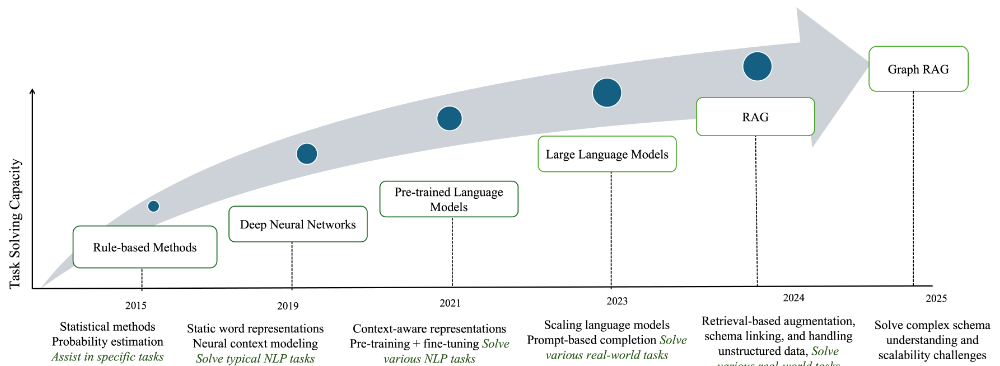
\includegraphics[width=\textwidth]{literature-review/text-to-sql-method-evolution.png}
      \caption{Краткая история развития моделей Text-to-SQL}
      \label{fig:text-to-sql-method-evolution}
\end{figure}

\paragraph{Ранние системы и подходы, основанные на правилах (1970-е – 2000-е)}. Первые NLIDB,
появившиеся еще в 1970-х годах, такие как LUNAR и более поздние системы,
основанные на синтаксическом разборе и онтологиях, полностью полагались на вручную созданные грамматики,
словари и наборы правил. Эти системы были <<зажатыми>>, имели ограниченный словарный запас и
требовали значительных усилий для адаптации к каждой новой предметной области.
Их главным недостатком была низкая гибкость и неспособность справляться с лингвистической вариативностью и
неоднозначностью естественного языка~\cite{karimiNonEnglishNaturalLanguage2022,
      pazosr.ComparativeStudyCustomization2016, kimNaturalLanguageSQL2020,
      bradDatasetNeuralNatural2017, mohammadjafariNaturalLanguageSQL2025}.

\paragraph{Появление машинного обучения и нейронных сетей (2010-е)}. Первый прорыв произошел с
развитием глубокого обучения. Исследователи начали рассматривать задачу Text-to-SQL как задачу
машинного перевода. Появились модели на основе рекуррентных нейронных сетей (RNN), в частности,
архитектуры Sequence-to-Sequence (Seq2Seq) с механизмом внимания (attention),
которые обучались на размеченных данных~\cite{bradDatasetNeuralNatural2017, visperasModernTexttoSQLSemantic2023}.
Катализатором для бурного развития этого направления стало появление крупных аннотированных
наборов данных, таких как WikiSQL и, в особенности, Spider.
Это позволило создавать и объективно сравнивать более сложные и точные нейросетевые модели,
такие как TypeSQL и SyntaxSQLNet, которые учитывали структуру схемы базы данных и
показывали значительно лучшие результаты по сравнению с системами
на правилах~\cite{kimNaturalLanguageSQL2020, visperasModernTexttoSQLSemantic2023}.
Однако по-прежнему оставались проблемы, такие как обработка вложенных запросов,
обобщение на конкретную базу данных и сопоставление неоднозначного естественного языка со структурированным
SQL~\cite{mohammadjafariNaturalLanguageSQL2025}.

\paragraph{Эпоха больших языковых моделей (LLM) (2020-е -- настоящее время)}. Последние несколько лет
ознаменовались доминированием больших языковых моделей (LLM), таких как модели GPT-4,
PaLM и LLaMA, что привело к очередной смене парадигмы. LLM лучше справляются в задачах, требующих понимания
и генерации человекоподобного текста, часто без дополнительной настройки. Они лучше улавливают
сложные взаимосвязи между естественным языком и схемами базы данных~\cite{zhuLargeLanguageModel2024,
      mohammadjafariNaturalLanguageSQL2025}. Однако, несмотря на свой потенциал, эти подходы обычно сталкиваются с несколькими проблемами:
галлюцинации моделей, неконтролируемый результат, высокое требование к вычислительным ресурсам.

С появлением LLM, разработка новых решений для задачи Text-to-SQL показала
заметную тенденцию к росту с сентября 2023 по октябрь 2024 года,
что свидетельствует о значительном интересе со стороны сообщества.
Количество публикаций достигло пика с июля по октябрь 2024 года,
составив примерно 39\% от общего их числа на тему
LLM-основанных методов решения Text-to-SQL.
Ожидается, что текущие достижения в этой области приведут к последующим инновациям
в методах преобразования текста в SQL. Эти достижения позиционируют LLM как
основу современных систем преобразования естественного языка в SQL,
устраняя разрыв между разговорными и формальными языками с растущей точностью и
эффективностью~\cite{huangExploringLandscapeTexttoSQL2025}.

\subsection{Текущее положение в исследованиях подходов к решению задачи Text-to-SQL
      с помощью моделей, основанных на LLM}

Как упоминается в источнике~\cite{huangExploringLandscapeTexttoSQL2025},
современные научные статьи в области Text-to-SQL можно классифицировать
следующим образом:
\begin{compactitem}
      \item Методологии
      \begin{compactitem}
            \item Предобработка (Pre-Processing)
            \item Обучение в контексте (In-context learning)
            \item Тонкая настройка (Fine-Tuning)
            \item Постобработка (Post-Processing)
      \end{compactitem}
      \item Наборы данных (Datasets)
      \item Метрики применения (Evaluation Metrics)
\end{compactitem}

\noindent Рассмотрим каждый вопрос, рассматриваемый в академической литературе по-отдельности.

\subsubsection{Методологии}

Как уже было отмечено, современные подходы к решению задачи Text-to-SQL в основном опираются
на большие языковые модели. Однако сами по себе LLM не являются готовым решением и
требуют применения целого ряда инженерных практик и методологий для достижения
высокой точности и эффективности. Исследователи~\cite{huangExploringLandscapeTexttoSQL2025}
выделяют четыре основных парадигмы, в рамках которых ведутся разработки и улучшения
LLM-основанных систем: предварительная обработка (Pre-Processing),
обучение в контексте (In-context learning), тонкая настройка (Fine-Tuning) и
постобработка (Post-Processing), что охватывает весь жизненный цикл обработки языка.
Это можно продемонстрировать с иллюстрации (см.~рис.~\ref{fig:llm-query-pipeline}).

\begin{figure}[!ht]
      \centering
      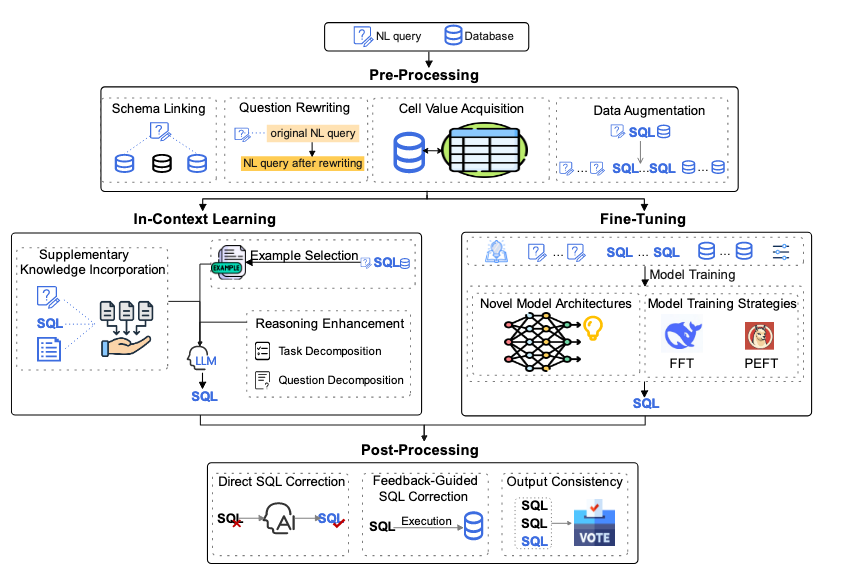
\includegraphics[width=\textwidth]{literature-review/llm-query-pipeline.png}
      \caption{Блок-схема типового конвейера обработки запроса в современной LLM-системе.}
      \label{fig:llm-query-pipeline}
\end{figure}


\subsubsection{Предварительная обработка (Pre-Processing)}

Этот этап является ключевым
для подготовки и структурирования входных данных, что напрямую влияет на точность
генерируемого SQL-запроса. Основная задача здесь --- максимально снизить неоднозначность
и предоставить модели всю необходимую для работы информацию.
Одним из центральных методов является \textit{связывание со схемой} (Schema Linking), в
ходе которого система сопоставляет слова и фразы из естественного языка с конкретными таблицами,
столбцами и их отношениями в базе данных~\cite{huangExploringLandscapeTexttoSQL2025,
      mohammadjafariNaturalLanguageSQL2025}. Другой важный метод --- \textit{извлечение значений ячеек}
(Cell Value Acquisition), который позволяет обогатить контекст, добавив в него
релевантные примеры значений из базы данных, что особенно полезно, когда в запросе
пользователя отсутствуют детали, необходимые для точной генерации
SQL~\cite{huangExploringLandscapeTexttoSQL2025}. Наконец, для борьбы с присущей
естественному языку двусмысленностью применяется \textit{переписывание вопроса}
(Question Rewriting), где модель сначала переформулирует исходный запрос в более
четкий и однозначный, прежде чем приступать к генерации кода.

\subsubsection{Обучение в контексте (In-Context Learning, ICL)}

Данная парадигма
сосредоточена на инженерии промптов (prompt engineering) --- искусстве составления
такого запроса к модели, который бы наиболее эффективно направлял ее на решение конкретной
задачи без необходимости изменять веса самой модели. Основные подходы
здесь --- это \textit{Zero-shot} (без примеров) и \textit{Few-shot}
(с малым количеством примерам)~\cite{zhuLargeLanguageModel2024}. В последнем случае ключевую
роль играет стратегия отбора примеров.
Для решения нетривиальных задач применяется \textit{усиление рассуждений}
(Reasoning Enhancement), где используются такие техники, как <<цепочка мыслей>>
(Chain-of-Thought, CoT)~\cite{zhuLargeLanguageModel2024,
      huangExploringLandscapeTexttoSQL2025}.

\subsubsection{Тонкая настройка (Fine-Tuning, FT)}

В отличие от ICL, этот метод предполагает
изменение весов предобученной модели путем ее дообучения на специфичном для задачи наборе данных.
Это позволяет создавать более специализированные и точные модели, особенно когда
используются LLM с открытым исходным кодом (open-source). Выделяют два основных
подхода: \textit{полная тонкая настройка} (Full Fine-Tuning, FFT), когда обновляются
все параметры модели, и \textit{параметрически-эффективная тонкая настройка}
(Parameter-Efficient Fine-Tuning, PEFT), при которой изменяется лишь небольшая
часть весов.
Второй подход позволяет значительно сократить вычислительные ресурсы, необходимые для
дообучения~\cite{huangExploringLandscapeTexttoSQL2025}.

Отличия в методологиях ICL и FT можно визуализировать с помощью иллюстрации (см.~рис.~\ref{fig:icl-vs-ft}).

\begin{figure}[h]
      \centering
      \begin{subcaptiongroup}
            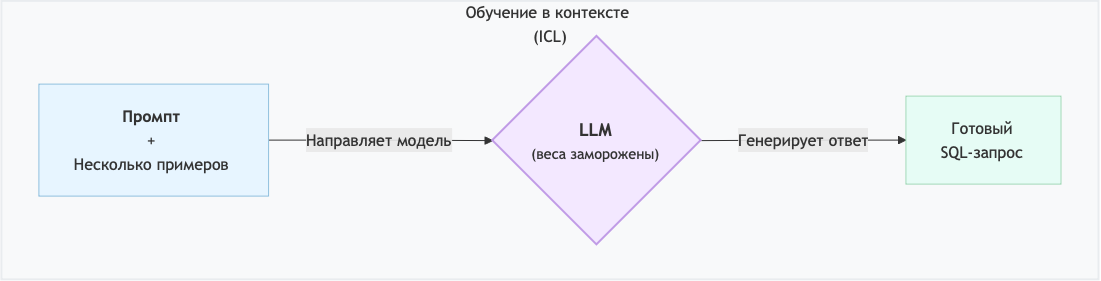
\includegraphics[width=\textwidth]{created-diagrams/icl-process.png}
            \caption{Процесс обучения в контексте (ICL)}
            \label{fig:icl-process}
            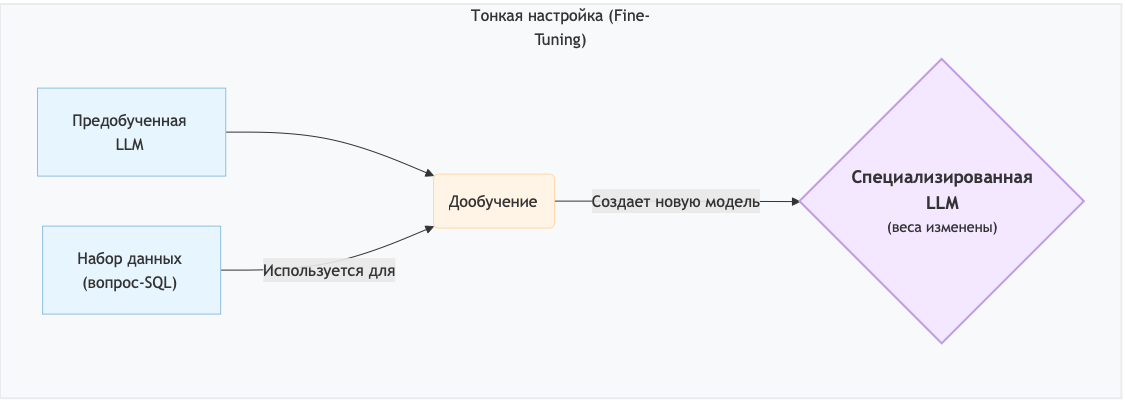
\includegraphics[width=\textwidth]{created-diagrams/ft-process.png}
            \caption{Процесс тонкой настройки (FT)}
            \label{fig:ft-process}
      \end{subcaptiongroup}
      \captionsetup{subrefformat=parens}
      \caption{Концептуальная схема, сравнивающая In-Context Learning и Fine-Tuning.}
      \label{fig:icl-vs-ft}
\end{figure}

\subsubsection{Постобработка (Post-Processing)}

Даже самые продвинутые модели могут генерировать
SQL-запросы с синтаксическими или логическими ошибками. Парадигма постобработки нацелена на
их исправление и верификацию. Один из подходов --- \textit{прямая коррекция SQL}, когда
модель сама или по заготовленным правилам ищет и исправляет ошибки в сгенерированном коде.
Более продвинутый метод --- \textit{коррекция на основе обратной связи}
(Feedback-Guided SQL Correction). В этом случае сгенерированный SQL-запрос выполняется в
базе данных, и если возникает ошибка, ее текст вместе с исходным запросом подается в модель
для повторной генерации~\cite{huangExploringLandscapeTexttoSQL2025}. Такой итеративный
подход реализован во многих современных системах, например, в компоненте Refiner системы
XiYan-SQL~\cite{gaoPreviewXiYanSQLMultiGenerator2025} или в агентных системах, таких как
MAC-SQL~\cite{zhuLargeLanguageModel2024}. Наконец, для повышения надежности используется
\textit{проверка согласованности вывода} (Output Consistency): система генерирует несколько
вариантов SQL-запроса, а затем выбирает наиболее вероятный или наиболее согласованный из них,
что является центральной идеей ансамблевого подхода в
XiYan-SQL~\cite{gaoPreviewXiYanSQLMultiGenerator2025, huangExploringLandscapeTexttoSQL2025}.

\subsubsection{Наборы данных (Datasets)}

Для обучения и объективной оценки моделей Text-to-SQL
необходимы качественные и разнообразные наборы данных.
Их развитие шло параллельно с эволюцией самих моделей,
от небольших и узкоспециализированных до масштабных и сложных.
Современные датасеты, как отмечается в~\cite{huangExploringLandscapeTexttoSQL2025},
можно разделить на несколько категорий.

Во-первых, это \textit{однодоменные} (single-domain) наборы данных,
такие как ATIS или GeoQuery, которые ориентированы на конкретную предметную
область и используются для оценки производительности моделей в узких задачах.
Во-вторых, что более актуально для
современных исследований, это \textit{междоменные} (cross-domain) датасеты.
Они требуют от моделей способности к обобщению, то есть умения работать с базами данных,
схемы которых не были представлены на этапе обучения. Ключевым датасетом в этой категории
является Spider~\cite{kimNaturalLanguageSQL2020, visperasModernTexttoSQLSemantic2023},
который стал отраслевым стандартом для оценки сложности и точности. Более поздние разработки,
такие как BIRD~\cite{huangExploringLandscapeTexttoSQL2025}, еще больше усложнили задачу,
добавив требования к обработке <<грязных>> данных и пониманию их семантики.

Помимо этого, выделяют и более специализированные
категории~\cite{huangExploringLandscapeTexttoSQL2025}:
\textit{контекстно-зависимые} (context-dependent) для оценки диалоговых систем,
\textit{ориентированные на робастность} (robustness-centered), которые проверяют
устойчивость моделей к синонимам и другим вариациям в
запросах и \textit{межъязыковые} (cross-lingual) для оценки качества работы с
неанглоязычными запросами. Именно наличие таких комплексных и
многоаспектных датасетов стимулирует исследователей к разработке все более совершенных моделей,
способных работать в условиях, приближенных к реальным~\cite{mohammadjafariNaturalLanguageSQL2025,
      gaoPreviewXiYanSQLMultiGenerator2025}.

\subsubsection{Метрики применения (Evaluation Metrics)}

Для количественной оценки
качества работы Text-to-SQL систем используются две основные группы
метрик~\cite{huangExploringLandscapeTexttoSQL2025}.

Первая группа~--- это метрики,
основанные на \textit{сопоставлении содержимого} (Content Matching-based).
Простейшей из них является \textit{точность полного совпадения строк} (Exact Matching Accuracy),
которая требует, чтобы сгенерированный SQL-запрос был посимвольно идентичен эталонному.
Это очень строгая метрика, которая не учитывает, что один и тот же результат можно
получить с помощью синтаксически разных, но семантически эквивалентных запросов.
Более гибкий подход предлагает \textit{точность совпадения компонентов} (Component-Match Accuracy),
используемая в бенчмарке Spider. Она разбивает SQL-запрос на
составные части (SELECT, WHERE, GROUP BY и т.д.) и оценивает корректность
каждой из них по-отдельности.

Вторая, и более важная с практической точки зрения, группа~--- это метрики,
основанные на \textit{результате выполнения} (Execution Result-based).
Ключевой метрикой здесь является \textit{точность выполнения} (Execution Accuracy, EX).
Она оценивает не синтаксическую схожесть запросов, а идентичность результатов,
полученных при выполнении сгенерированного и эталонного SQL-запросов на базе данных.
Именно эта метрика является основной в большинстве современных исследований и бенчмарках,
включая BIRD и Spider, так как она напрямую отражает способность системы дать
пользователю правильный ответ~\cite{huangExploringLandscapeTexttoSQL2025,
      gaoPreviewXiYanSQLMultiGenerator2025}.


\subsection{Выбор и обоснование базовой системы для реализации NLIDB}
Для практической реализации собственного естественно-языкового интерфейса в рамках
УИР необходимо выбрать конкретную систему или фреймворк,
который будет служить технологическим ядром. Выбор должен основываться на
объективных показателях производительности, архитектурном соответствии современным
тенденциям и практической применимости для решения поставленных задач.

В качестве такой системы была выбрана XiYan-SQL~--- современный ансамблевый фреймворк,
разработанный исследователями из Alibaba Group\cite{gaoPreviewXiYanSQLMultiGenerator2025}.
Данное решение представляет собой комплексный подход,
объединяющий несколько передовых методологий, рассмотренных ранее.

Выбор в пользу XiYan-SQL обусловлен несколькими причинами:

\paragraph{Лидирующие позиции в ключевых бенчмарках}. На момент проведения исследования XiYan-SQL
занимает первые места в наиболее авторитетных и сложных междоменных бенчмарках,
таких как Spider и BIRD.
Согласно данным с ресурса <<Papers with Code>>
\footnote{URL: \url{https://paperswithcode.com}}, данный фреймворк демонстрирует
лучшие результаты по метрике Execution Accuracy,
опережая другие известные системы. Графически его лидирование может быть проиллюстрировано
на графиках (см.~рис.~\ref{fig:SOTA-Spider-Bird}).
Это является объективным подтверждением
его высокой точности и способности генерировать корректные SQL-запросы
для разнообразных баз данных.

\paragraph{Современная гибридная архитектура}. С архитектурной точки зрения,
XiYan-SQL реализует передовой ансамблевый подход,
который сочетает сильные стороны как тонкой настройки,
так и обучения в контексте.
Система использует несколько генераторов~--- часть из них дообучена
для генерации высокоточных и стилистически разнообразных запросов,
а другая часть использует ICL для повышения гибкости.
Такой подход позволяет достичь баланса между точностью,
разнообразием и способностью справляться со сложными запросами.
Кроме того, в фреймворк встроены механизмы постобработки (Refiner) и
отбора лучших запросов, что полностью соответствует передовым подходам,
описанным в академической литературе~\cite{gaoPreviewXiYanSQLMultiGenerator2025,
      huangExploringLandscapeTexttoSQL2025}.

\paragraph{Практическая доступность и применимость}. Немаловажным фактором,
особенно в рамках академической работы, является практическая доступность фреймворка.
Разработчики XiYan-SQL предоставили открытый доступ к исходному коду своей системы
через репозиторий на GitHub \footnote{URL: \url{https://github.com/XGenerationLab/xiyan_mcp_server}}.
Это позволяет не просто теоретически изучить подход,
но и интегрировать его в собственный проект, адаптировать и использовать в качестве
основы для дальнейших разработок. Это значительно снижает порог вхождения и позволяет
сконцентрироваться на задачах более высокого уровня, таких как разработка
пользовательского интерфейса и логики работы веб-сервиса.

\paragraph{Соответствие задачам исследования}. На начальном этапе данная
курсовая работа предполагает создание NLIDB для работы с отдельными,
не связанными между собой таблицами. Иначе говоря, с реляционными базами данных,
состоящих из единственных таблиц. Хотя XiYan-SQL способен обрабатывать и
более сложные межтабличные запросы,
его фундаментальная точность и робастность являются отличной основой и для более
простых сценариев.

При выборе были рассмотрены и другие системы,
представленные в таблицах лидеров отраслевых бенчмарков (см.~рис.~\ref{fig:SOTA-Spider-Bird}).
Однако многие из них либо показывают более низкую производительность на
комплексных датасетах, либо представляют собой более ранние архитектурные решения,
либо не предоставляют готового к внедрению открытого кода, что делает их
использование в рамках данного проекта нецелесообразным.

Важно отметить, что данный выбор касается именно технологического ядра
для преобразования текста в SQL. Вопрос о новизне и актуальности создания
нового веб-сервиса с подобным функционалом требует отдельного анализа
существующих коммерческих и открытых продуктов, который будет проведен
на следующем этапе работы. Тем не менее, для решения центральной
задачи~--- качественной трансляции естественного языка в SQL~--- фреймворк
XiYan-SQL на сегодняшний день является наиболее мощным, современным и подходящим.




\section{Обзор существующих веб-сервисов и обоснование актуальности разработки собственного веб-сервиса}

\begin{annotation}
      В данном разделе представлен обзор существующих веб-сервисов, реализующих естественно-языковой
      интерфейс к базам данных (NLIDB), включая как проприетарные, так и решения с открытым исходным кодом.
      На основе сравнительного анализа выявляются основные
      ограничения современных решений и обосновывается актуальность
      разработки собственного веб-сервиса с NLIDB.
\end{annotation}

После выбора передового технологического ядра в лице фреймворка XiYan-SQL,
необходимо провести анализ существующих на рынке веб-сервисов, предоставляющих
функциональность естественно-языкового интерфейса к базам данных (NLIDB).
Этот анализ позволит определить, существуют ли готовые решения, полностью
удовлетворяющие потребностям целевой аудитории, и выявить незанятые ниши,
что в свою очередь обоснует актуальность и научную новизну данного проекта.
Для этого был проведен обзор нескольких популярных веб-сервисов и
open-source решений.

\subsection{Обзор существующих веб-сервисов с интеграцией ИИ для упрощения
      взаимодействия с базами данных}

\paragraph{WrenAI}. Это мощная платформа, которая существует в двух вариантах:
облачный коммерческий сервис (Wren Cloud) и решение с открытым исходным кодом
для самостоятельного развертывания (WrenAI Open Source)
\footnote{URL: \url{https://docs.getwren.ai/oss/overview/introduction}}.
Система позволяет создавать как собственные базы данных (CSV), так и напрямую подключаться к
широкому спектру реляционных баз данных. Ключевым недостатком для нетехнического
пользователя является необходимость локальной установки и настройки open-source версии,
что требует определенных технических навыков. Кроме того, система в своей основе полагается
на API от OpenAI, что создает барьер для пользователей из России и повышает зависимость
от стороннего платного сервиса. Пользовательский интерфейс, хоть и функциональный, может
показаться перегруженным для базовых задач.

\paragraph{SQLAI}. Данный сервис позиционируется как многофункциональный инструмент,
ориентированный не только на конечных пользователей, но и на разработчиков
\footnote{URL: \url{https://www.sqlai.ai/documentation/introduction/introduction}}.
Он предлагает генерацию SQL-запросов, их оптимизацию и отладку. Важным преимуществом
является поддержка не только реляционных, но и некоторых NoSQL баз данных. Однако, это
полностью коммерческий продукт с закрытым исходным кодом, что делает невозможным его
кастомизацию и изучение внутреннего устройства. Англоязычный интерфейс и широкий, но
избыточный для нетехнического специалиста функционал, делают его менее подходящим для
целей нашего исследования.

\paragraph{ai2sql}. Этот сервис сфокусирован на простоте и предлагает интуитивно
понятный интерфейс для преобразования запросов на естественном языке в SQL
\footnote{URL: \url{https://ai2sql.io}}. Он поддерживает работу с загружаемыми CSV-файлами,
что является удобным сценарием для пользователей, не имеющих прямого доступа к базам данных.
Как и предыдущий аналог, ai2sql является проприетарным решением с закрытым исходным кодом и
англоязычным интерфейсом, что ограничивает его применимость и прозрачность.

\paragraph{SQLchat}. SQLchat~--- это проект с открытым исходным кодом,
который предоставляет веб-интерфейс для <<общения>> с базой данных
\footnote{URL: \url{https://www.sqlchat.ai}}. Его основное преимущество~--- открытость и простота.
Однако, он не поддерживает загрузку данных из файлов (например, CSV) и требует от пользователя
прямого подключения к уже существующей и настроенной базе данных, что может быть барьером для
целевой аудитории.

\paragraph{AI SQL Gen}. Данный проект является типичным примером простой системы-обертки над
GPT-4 \footnote{URL: \url{https://github.com/marblexyz/aisqlgen}}, что наглядно демонстрирует его
архитектура (см.~рис.~\ref{fig:aisqlgen_arch}). Он требует от пользователя
наличия собственного ключа OpenAI API, запускается локально и не обновлялся в течение долгого
времени. Несмотря на простоту, такие системы полностью зависят от стороннего сервиса и не
предлагают никакой дополнительной ценности в виде продвинутого связывания со схемой или
поддержки различных моделей.

\begin{figure}[ht]
      \begin{center}
            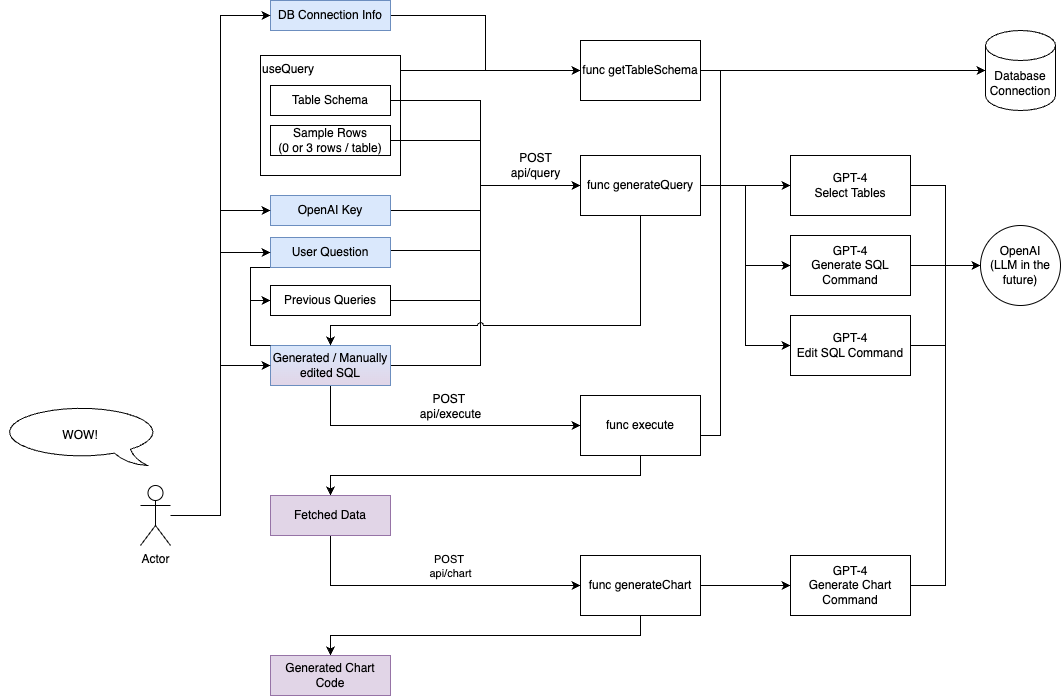
\includegraphics[width=0.9\textwidth]{literature-review/aisqlgen-diagram.png}
      \end{center}
      \caption{Архитектура типичной системы-обертки (на примере AI SQL Gen)}
      \label{fig:aisqlgen_arch}
\end{figure}

\subsection{Сравнительный анализ и обоснование актуальности собственной разработки}

Проведенный обзор позволяет систематизировать существующие решения и выявить их
ключевые характеристики, которые представлены в виде сравнительной таблицы
(см.~табл.~\ref{table:services_comparison}).

\begin{table}[ht]
      \caption{Сравнительная таблица существующих NLIDB-сервисов}\label{table:services_comparison}
      \begin{tabularx}{\linewidth}{|>{\bfseries}l|X|X|X|}
            \hline
            \textbf{Сервис} & \textbf{Модель развертывания}                              & \textbf{Подключение данных}                & \textbf{Модель монетизации и API}                             \\
            \hline
            WrenAI          & Open-source (локальный) или проприетарный веб-сервис Cloud & CSV, прямое подключение к БД               & Требует ключ OpenAI API при использовании open-source решения \\
            \hline
            SQLAI.ai        & Проприетарный веб-сервис                                   & Прямое подключение к БД (SQL     \& NoSQL) & Коммерческий, закрытый исходный код                           \\
            \hline
            ai2sql.io       & Проприетарный веб-сервис                                   & Загрузка CSV, прямое подключение           & Коммерческий, закрытый исходный код                           \\
            \hline
            SQLchat         & Open-source (локальный)                                    & Только прямое подключение к БД             & Бесплатный, с открытым кодом, требует ключ OpenAI API         \\
            \hline
            AI SQL Gen      & Open-source (локальный)                                    & Только прямое подключение к БД             & Требует ключ OpenAI API                                       \\
            \hline
      \end{tabularx}
\end{table}

Анализ таблицы и детальный обзор сервисов позволяет сделать несколько ключевых выводов
и выявить недостатки у альтернативых решений, что и обосновывает актуальность в собственной разработке
веб-сервиса в рамках УИР.

\begin{compactitem}
      \item \textbf{Проблема доступности}. На рынке наблюдается четкое разделение:
      либо платные, закрытые веб-сервисы, либо open-source проекты,
      требующие от пользователя технических навыков для локального развертывания.
      Практически отсутствует ниша веб-сервиса, который был бы одновременно
      с открытым исходным кодом, бесплатным для конечного пользователя и доступным онлайн
      без необходимости установки.
      \item \textbf{Зависимость от проприетарных API}. Большинство доступных решений,
      включая open-source, жестко привязаны к API коммерческих LLM, в первую очередь~--- OpenAI.
      Это создает существенный барьер для пользователей из России
      (из-за сложностей с оплатой и регистрацией) и повышает риски,
      связанные с конфиденциальностью данных, передаваемых на сторонние серверы.
      \item \textbf{Непрозрачность технологического ядра}. Коммерческие сервисы не раскрывают,
      какие модели и методы они используют <<под капотом>>. В то же время,
      многие простые open-source проекты используют базовые подходы без применения передовых техник.
      Создание сервиса на основе доказуемо лидирующего фреймворка, такого как XiYan-SQL,
      является важным преимуществом с точки зрения научной и инженерной проработки.
\end{compactitem}

Таким образом, выявлена четкая потребность в создании веб-сервиса с открытым исходным кодом,
который не требует от конечного пользователя сторонних API-ключей,
прост в использовании и основан на современной, высокопроизводительной модели для
генерации SQL-запросов. Разработка такого продукта не только представляет
академический интерес как пример интеграции лидирующей модели в прикладной инструмент,
но и обладает высокой практической ценностью, предлагая рынку уникальное и востребованное решение.
Это и определяет актуальность и новизну дальнейшей работы.




\section{Выводы}

В рамках данного исследования был проведен комплексный анализ проблематики
взаимодействия нетехнических пользователей с базами данных,
а также обзор и сравнение существующих подходов и технологий для решения этой проблемы.
Основной целью анализа было создание концепта итогового продукта при
разработке собственного естественно-языкового интерфейса, а также проверка его актуальности и
новизны подходов.
По результатам проделанной работы
были сделаны следующие ключевые выводы, которые определяют дальнейший ход проекта:

\begin{compactenum}
      \item Выявлена проблема возникновения трудностей у нетехнических пользователей
      при взаимодействии с базами данных. Анализ традиционных
      способов взаимодействия с базами данных однозначно
      показал, что все они требуют от пользователя наличия специальных технических знаний,
      что и является основным препятствием для нетехнических специалистов.
      \item Проделан сравнительный анализ адаптированных пользовательских
      интерфейсов. На основании преимуществ и недостатков таких интерфейсов, как QBE, VQS или
      NLIDB~--- был сделан вывод,
      что именно естественно-языковые интерфейсы (NLIDB) являются наиболее перспективным направлением,
      так как они предлагают самый высокий уровень абстракции и интуитивности,
      полностью скрывая от пользователя сложность структуры данных и синтаксиса формальных языков,
      что дало повод сконцентрироваться на исследовании именно такого вида взаимодействия с БД.
      \item Определена доминирующая технология. Глубокий анализ систем,
      решающих задачу преобразования естественного языка в SQL (Text-to-SQL),
      показал четкую эволюцию от ранних систем на правилах к современным решениям на
      основе больших языковых моделей (LLM). Было установлено, что лучшую
      производительность сегодня демонстрируют гибридные LLM-основанные фреймворки,
      которые комбинируют различные методологии
      для достижения максимальной точности и робастности при решении исходной задачи.
      \item Выбрано конкретное технологическое ядро. На основе анализа производительности,
      архитектурных особенностей и практической доступности был выбран фреймворк XiYan-SQL
      в качестве базовой системы для реализации собственного NLIDB. Этот выбор обоснован его лидирующими
      позициями в ключевых отраслевых бенчмарках, современной ансамблевой архитектурой,
      а также наличием открытого исходного кода, что позволяет интегрировать его в собственный проект.
      \item Обоснована актуальность и новизна разработки.
      Было установлено, что на данный момент практически отсутствуют веб-сервисы, которые
      бы одновременно являлись:
      \begin{compactitem}
            \item Полностью бесплатными и доступными онлайн без локальной установки.
            \item Основанными на открытом исходном коде.
            \item Не требующими от конечного пользователя предоставления собственных API-ключей
            к платным проприетарным LLM.
      \end{compactitem}
\end{compactenum}

Таким образом, результаты анализа, проведенного в данной части УИР, подтвердили актуальность
поставленной задачи и позволили сформировать план
для ее решения. Дальнейшая работа будет сконцентрирована на проектировании, разработке и
тестировании собственного веб-сервиса, который будет использовать фреймворк XiYan-SQL в качестве
ядра для трансляции запросов, предоставляя доступный, бесплатный и прозрачный инструмент для
широкого круга нетехнических пользователей.




\section{Цели и задачи на УИР}

Целью данного УИР является проектирование модели интеграции современного многомодульного
NLIDB-ядра XiYan-SQL во внешний веб-сервис. Эта интеграция достигается через разработку
архитектуры компонента-оркестратора, а именно \textbf{MCP-клиента}, который инкапсулирует
всю сложность взаимодействия с ядром.

Практической апробацией предложенной модели служит разработка и
тестирование программного прототипа веб-сервиса. На данном этапе исследования
прототип \textbf{эмулирует} взаимодействие с ядром XiYan-SQL, что позволяет проверить
корректность и жизнеспособность спроектированной архитектуры в контролируемой среде.

Для достижения поставленной цели необходимо решить следующие задачи:
\begin{compactenum}
      \item Проанализировать архитектуру и протокол взаимодействия многоагентного сервера
      XiYan-SQL MCP Server для определения требований к клиентской части.
      \item Спроектировать логику работы (модель взаимодействия) MCP-клиента,
      определяющую полный жизненный цикл обработки пользовательского запроса.
      Это включает последовательность вызовов к различным AI-агентам ядра: агенту связывания со
      схемой, генераторам кандидатов и агенту выбора конечного результата.
      \item Определить внутренний API компонента MCP-клиента для его взаимодействия с
      остальными частями серверной логики веб-приложения.
      \item Спроектировать общую клиент-серверную архитектуру веб-сервиса,
      который предоставляет пользователю интерфейс для выполнения запросов к
      базам данных на естественном языке.
      \item Разработать программный прототип веб-сервиса, реализующий спроектированную архитектуру.
      Прототип должен включать серверную часть (Backend), пользовательский интерфейс (Frontend) и,
      самое главное, модуль MCP-клиента с \textbf{эмуляцией} вызовов к ядру XiYan-SQL.
      \item Провести функциональное тестирование разработанного прототипа для проверки
      корректности работы реализованной модели взаимодействия MCP-клиента и
      пользовательского интерфейса.
\end{compactenum}

\clearpage

 \chapter{Разработка моделей и алгоритмов \dots}

В этой главе описываются разработанные/модифицированные модели/методы/
алгоритмы, или/и описывается применение известных стандартных методов. Также, 
в конце главы обычно приводится общая архитектура программной системы, 
вытекающая из описанной теории. Приведенные ниже заголовки подразделов так же 
весьма примерные и сильно зависят от особенностей конкретной работы.

Формулы и их части необходимо набирать в математическом режиме
(символ \verb|$|). Во избежание переноса длинных формул между строками их 
стоит размещать по центру колонки, например,
\begin{center}
$S a b c = (\lambda x y z. x z (y z)) a b c = a c (b c)$,
\end{center}
\noindent и, если абзац после формулы продолжается, необходимо использовать 
\verb|\noindent|.

Для набора правил вывода можно использовать пакет \texttt{mathpartir.sty}. 
Правила вывода могут быть вынесены в виде рисунка (см. рис. 
\ref{img:inferrules}).

\begin{figure}[t]
  \centering
    \begin{mathpar}
      \inferrule{
        M \to M'
      }{
        N M \to N M'
      } \quad (\mu) \and 
      \inferrule{
        M \to M'
      }{
        M N \to M' N
      } \quad (\nu) \and
      \inferrule{
        M \to M'
      }{
        \lambda x. M \to \lambda x. M'
      } \quad (\xi)
    \end{mathpar}
  \caption{Правила редукции}
  \label{img:inferrules}
\end{figure}

Для оформления определений, теорем, доказательств и т.~п. могут быть 
использованы соответствующие окружения, например:

\begin{definition}
(высказывание)
Высказыванием называется любое истинное или ложное утверждение.
\end{definition}


\section{Модель системы \dots}

\dots




\section{Метод решения задачи для \dots}

\dots





\section{Алгоритмы вычисления \dots}

\dots





\section{Обобщенная архитектура и интерфейсы \dots}

В ряде случаев, все или некоторые результаты проектирования могут быть представлены во второй главе. Обычно же архитектура описывается в третьей главе.

\section{Выводы}

Необходимо перечислить, какие теоретические результаты были получены с 
указанием степени новизны. Например: <<Была разработана такая-то модель. Она 
представляет собой адаптированную версию модели $X$, в которой уравнение $Z$ 
заменено на уравнение $Z'$>>. Еще пример: <<Была предложена такая-то 
архитектура, она отличается от типовой в том-то и том-то. Это позволяет 
избежать таких-то проблем.>>. При этом не следует заниматься <<высасыванием из 
пальца>>: <<Поставленная задача является типовой; для ее решения применены 
стандартные средства (перечислить, какие).>>.


\clearpage

\chapter{Проектирование и программная реализация прототипа веб-сервиса}
\label{chapter3}

\begin{annotation}
      В данной главе описывается процесс проектирования и программной реализации прототипа веб-сервиса с естественно-языковым интерфейсом. На основе сформулированных в предыдущей главе требований, с использованием языка моделирования UML, разрабатывается архитектура системы. Представляются диаграммы вариантов использования, компонентов и последовательности, которые детально описывают как статическую структуру, так и динамику взаимодействия элементов системы. В завершение приводится описание выбранного технологического стека и ключевых аспектов реализации прототипа.
\end{annotation}

\section{Проектирование архитектуры системы с использованием UML}

Проектирование является критически важным этапом разработки любого программного продукта. Для визуализации и формализации архитектуры будущего веб-сервиса был использован унифицированный язык моделирования UML (Unified Modeling Language). Были построены три диаграммы, описывающие систему с разных уровней абстракции.

\subsection{Диаграмма вариантов использования (Use Case Diagram)}

Диаграмма вариантов использования является наиболее высокоуровневым представлением системы. Она определяет границы системы, ее основных действующих лиц (акторов) и цели, которые эти акторы могут достигать при взаимодействии с системой.

Для нашего веб-сервиса был определен один актор~--- \textbf{Пользователь}. Его основные цели (варианты использования) представлены на рис.~\ref{fig:use-case-diagram}.

\begin{figure}[ht]
      \centering
      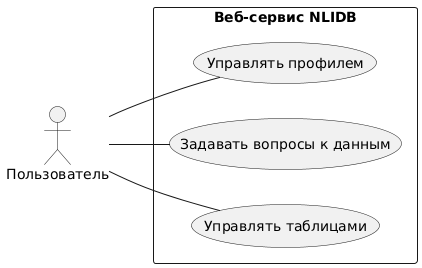
\includegraphics[width=0.7\textwidth]{created-diagrams/uml/use-case-diagram.png}
      \caption{Диаграмма вариантов использования}
      \label{fig:use-case-diagram}
\end{figure}

Как видно из схемы, Пользователь может выполнять три ключевые функции:
\begin{compactitem}
      \item \textbf{Управлять таблицами}. Этот вариант использования включает в себя загрузку
      новых таблиц (CSV/Excel), их переименование и удаление, а также добавление
      описаний для столбцов.
      \item \textbf{Задавать вопросы к данным}. Основная функция системы,
      позволяющая пользователю формулировать запросы на естественном языке к выбранной таблице.
      \item \textbf{Управлять профилем}. Включает в себя регистрацию, аутентификацию и
      изменение данных своего аккаунта (псевдоним, пароль, аватар).
\end{compactitem}

\subsection{Диаграмма компонентов (Component Diagram)}

Диаграмма компонентов описывает физическую структуру системы, показывая,
из каких крупных программных блоков она состоит и как они связаны между собой.
Эта диаграмма является основной архитектурной схемой нашего веб-сервиса
(см.~рис.~\ref{fig:component-diagram}).

\begin{figure}[ht]
      \centering
      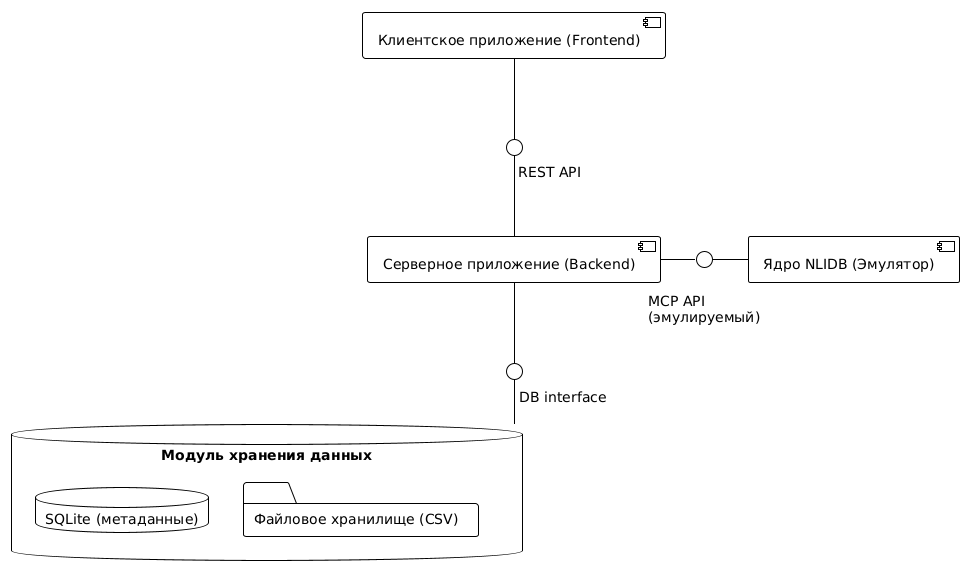
\includegraphics[width=1\textwidth]{created-diagrams/uml/component-diagram.png}
      \caption{Диаграмма компонентов системы}
      \label{fig:component-diagram}
\end{figure}

Система состоит из четырех основных компонентов:
\begin{compactenum}
      \item \textbf{Клиентское приложение (Frontend):} Компонент, работающий в браузере пользователя.
      Реализован на HTML/CSS/JS. Отвечает за пользовательский интерфейс и взаимодействие с
      бэкендом через REST API.
      \item \textbf{Серверное приложение (Backend):} Основной компонент, реализованный на
      Python с использованием фреймворка FastAPI. Он предоставляет REST API,
      управляет бизнес-логикой и выступает в роли организатора для других компонентов.
      \item \textbf{Модуль хранения данных:} Отвечает за персистентное хранение информации.
      Он состоит из базы данных \textbf{SQLite} для метаинформации
      (пользователи, таблицы, описания столбцов) и \textbf{Файлового хранилища} для
      загруженных CSV/Excel файлов и аватаров пользователей.
      \item \textbf{Ядро NLIDB (Эмулятор):} В рамках прототипа~--- это компонент-эмулятор,
      имитирующий работу настоящего XiYan-SQL MCP Server. Он предоставляет внутренний API,
      который полностью соответствует спроектированному протоколу взаимодействия с целевой системой.
\end{compactenum}

\subsection{Диаграмма последовательности (Sequence Diagram)}

Диаграмма последовательности детализирует взаимодействие между компонентами во времени.
Она наглядно демонстрирует, какие вызовы и в какой последовательности происходят для
выполнения конкретного варианта использования. На рис.~\ref{fig:sequence-diagram} показана
последовательность действий для самого важного сценария~--- обработки запроса пользователя на
естественном языке.

\begin{figure}[ht]
      \centering
      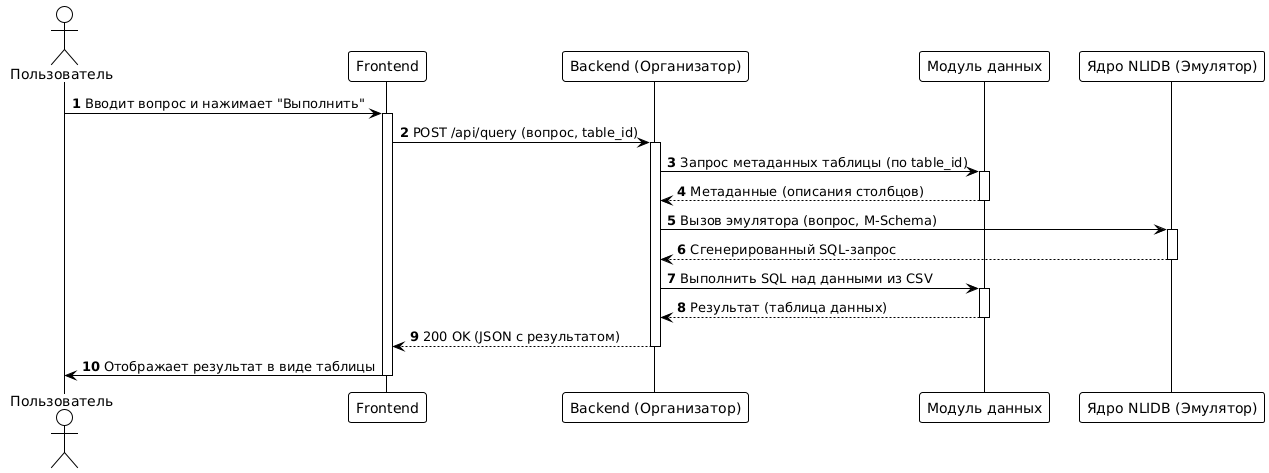
\includegraphics[width=\textwidth]{created-diagrams/uml/sequence-diagram.png}
      \caption{Диаграмма последовательности для обработки ЕЯ-запроса}
      \label{fig:sequence-diagram}
\end{figure}

Процесс, изображенный на диаграмме, состоит из следующих шагов:
\begin{compactenum}
      \item Пользователь вводит вопрос в интерфейсе и нажимает кнопку <<Выполнить>>.
      \item \textbf{Frontend} отправляет асинхронный \verb|POST| запрос на эндпоинт
      \verb|/api/query| \textbf{Backend}-сервера, передавая текст вопроса и ID выбранной таблицы.
      \item \textbf{Backend (Организатор)} получает запрос и\
      сначала обращается к \textbf{Модулю данных}, чтобы получить метаинформацию о таблице
      (путь к файлу, описания столбцов) из базы SQLite.
      \item Получив метаданные, \textbf{Backend} формирует из них M-Schema и
      обращается к \textbf{Ядру NLIDB (Эмулятору)}, передавая ему вопрос и схему.
      \item \textbf{Эмулятор} для тестовых сценариев возвращает заранее заготовленный SQL-запрос.
      \item \textbf{Backend} получает SQL. Он снова обращается к \textbf{Модулю данных},
      но на этот раз для выполнения операции: он считывает нужный CSV-файл в объект pandas
      DataFrame и выполняет над ним полученный SQL-запрос с помощью библиотеки \texttt{pandasql}.
      \item \textbf{Модуль данных} возвращает результат выполнения~--- новый DataFrame.
      \item \textbf{Backend} сериализует результирующий DataFrame в формат JSON и
      отправляет его обратно на \textbf{Frontend} в теле успешного HTTP-ответа.
      \item \textbf{Frontend} получает данные и отрисовывает их в виде таблицы для
      Пользователя.
\end{compactenum}

Данные диаграммы полностью описывают спроектированную архитектуру и
служат основой для этапа программной реализации.




\section{Выбор стека технологий}

На основе спроектированной в предыдущем разделе архитектуры был выбран конкретный стек
технологий для программной реализации прототипа. Выбор каждого инструмента и фреймворка
обусловлен функциональными требованиями проекта, необходимостью разработки прототипа и
возможностями для дальнейшего масштабирования системы.

\paragraph{Серверная часть (Backend)}. Для реализации серверной части был выбран язык
программирования \textbf{Python} и асинхронный веб-фреймворк \textbf{FastAPI}.
Этот выбор обусловлен следующими причинами:
\begin{compactitem}
      \item \textbf{Экосистема Python для ИИ и анализа данных}. Ключевое ядро системы,
      XiYan-SQL, написано на Python. Использование Python для бэкенда является наиболее
      нативным и эффективным решением, так как позволяет избежать сложностей межъязыкового
      взаимодействия и напрямую интегрировать необходимые библиотеки.
      \item \textbf{Высокая производительность FastAPI}. FastAPI построен на базе Starlette и Pydantic,
      что обеспечивает ему производительность, сопоставимую с решениями на Go и Node.js.
      Его асинхронная природа идеально подходит для обработки запросов, связанных с
      длительными операциями, такими как обращение к LLM.
      \item \textbf{Автоматическая документация API}. FastAPI автоматически генерирует
      интерактивную документацию для API (Swagger UI и ReDoc), что значительно упрощает
      процесс разработки, тестирования и отладки взаимодействия между клиентской и серверной частями.
      \item \textbf{Работа с данными}. Для манипуляции данными из загружаемых
      CSV-файлов используется библиотека \textbf{pandas}~--- де-факто стандарт для
      анализа данных в Python. Для выполнения SQL-запросов над объектами DataFrame
      используется библиотека \textbf{pandasql}, что позволяет обрабатывать данные из файлов так,
      как если бы они находились в реляционной базе данных.
\end{compactitem}

\paragraph{Клиентская часть (Frontend)}.
Для реализации пользовательского интерфейса был выбран базовый стек из
\textbf{HTML5, CSS3 и нативного JavaScript (Vanilla JS)} по следующим причинам:
\begin{compactitem}
      \item \textbf{Фокус на основной задаче}. Основная сложность и новизна проекта лежат в
      серверной части и архитектуре взаимодействия с NLIDB-ядром. Использование стандартного
      стека без тяжелых фреймворков (таких как React или Vue) позволяет сконцентрировать усилия
      на реализации ключевой функциональности.
      \item \textbf{Отсутствие зависимостей и простота развертывания}. Данный подход не требует
      сложной системы сборки и зависимостей (Node.js, npm), что упрощает разработку и
      развертывание прототипа.
      \item \textbf{Гибкость}. Спроектированный REST API полностью отделяет логику бэкенда от
      представления. Это означает, что в будущем клиентская часть может быть легко заменена на
      более современный фреймворк без каких-либо изменений в серверной архитектуре.
\end{compactitem}

\paragraph{База данных (Database)}.
Для хранения метаинформации (данные пользователей, сведения о загруженных таблицах и
описания столбцов) была выбрана легковесная встраиваемая СУБД \textbf{SQLite}. Вот причины, по
которым была выбрана именно она:
\begin{compactitem}
      \item \textbf{Серверная независимость}. SQLite не требует отдельного серверного процесса.
      База данных представляет собой один файл, что идеально подходит для прототипа и упрощает
      его переносимость и настройку.
      \item \textbf{Нативная поддержка в Python}. SQLite встроена в стандартную библиотеку Python,
      что избавляет от необходимости устанавливать внешние драйверы. Для удобной работы с базой
      данных используется \textbf{SQLAlchemy}~--- популярный ORM (Object-Relational Mapper),
      который позволяет работать с таблицами как с Python-объектами.
\end{compactitem}

Таким образом, выбранный технологический стек представляет собой сбалансированное решение,
которое позволяет быстро и эффективно реализовать прототип, полностью соответствующий
поставленным задачам, и при этом закладывает прочный фундамент для будущего развития и
усложнения системы.




\section{Описание программной реализации прототипа веб-сервиса}

На основе спроектированной архитектуры и выбранного стека технологий был реализован
программный прототип веб-сервиса. В данном разделе приводится описание ключевых модулей и
функций системы. Фрагменты исходного кода, иллюстрирующие реализацию, вынесены в приложение
(см.~прил.~\ref{appendix-B}).




\subsection{Описание реализованных функций и модулей}

Программный код проекта организован в модульную структуру, соответствующую современным
практикам разработки на FastAPI. Корневая директория содержит главный файл приложения
\verb|main.py|, файлы конфигурации и директории с различными компонентами системы:
\verb|api|, \verb|core|, \verb|db|, \verb|features|, \verb|services|.

\paragraph{Точка входа и конфигурация приложения}. Файл \verb|main.py| является точкой
входа в приложение. В нем создается экземпляр класса \verb|FastAPI|, настраиваются
middleware-компоненты (включая \verb|CORSMiddleware| для обработки кросс-доменных запросов),
монтируются директории для статических файлов (\verb|/static|) и загрузок (\verb|/uploads|),
а также подключаются все API-маршруты из модуля \verb|api|. Важной частью является функция
с жизненным циклом (\verb|lifespan|), которая при старте сервера создает необходимые директории,
например, для аватаров пользователей.

\paragraph{Модуль аутентификации и управления пользователями}.
Данная функциональность реализована в директории \verb|features/users/|.
\begin{compactenum}
      \item \textbf{Модель данных (\texttt{models.py})}. Описана модель \verb|User| с
      использованием SQLAlchemy ORM. Она содержит поля для хранения псевдонима,
      хэшированного пароля, URL аватара и флагов статуса пользователя (активен,
      суперпользователь, стандартный аватар).
      \item \textbf{Операции с данными (\texttt{crud.py})}. Реализован класс \verb|CRUDUser|,
      который инкапсулирует всю логику прямого взаимодействия с базой данных:
      создание пользователя, поиск по имени, аутентификация, обновление. Для хэширования
      паролей используется библиотека \verb|passlib| с алгоритмом bcrypt, что обеспечивает
      безопасное хранение учетных данных.
      \item \textbf{API эндпоинты (\texttt{api.py})}. Определены все публичные маршруты для
      работы с пользователями:
      \begin{compactenum}
            \item \verb|/register|: Регистрация нового пользователя с валидацией длины и
            формата псевдонима и пароля.
            \item \verb|/login/access-token|: Аутентификация пользователя и
            выдача JWT-токена доступа, который используется для авторизации всех
            последующих запросов.
            \item \verb|/me|, \verb|/me/username|, \verb|/me/password|: Маршруты для получения и
            обновления данных текущего пользователя.
            \item \verb|/me/avatar|: Эндпоинты для загрузки и удаления пользовательского аватара.
      \end{compactenum}
      \item \textbf{Сервис генерации аватаров (\texttt{services/avatar\_service.py})}. Выделенный
      сервис, который при регистрации или удалении кастомного аватара генерирует стандартное
      изображение с первой буквой псевдонима пользователя на цветном фоне, созданном на
      основе хэша от имени. Для генерации используется библиотека \verb|Pillow|.
\end{compactenum}

\paragraph{Модуль управления таблицами данных}.
Аналогично пользователям, логика работы с таблицами вынесена в модуль \verb|features/tables/|.
\begin{compactenum}
      \item \textbf{Модель данных (\texttt{models.py})}. Описана модель \verb|Table|,
      связанная с моделью \verb|User| отношением <<один-ко-многим>>. Хранит имя таблицы,
      оригинальное имя файла, путь к файлу на сервере и ID владельца.
      \item \textbf{Сервис обработки таблиц (\texttt{services/table\_service.py})}. Этот
      сервисный слой содержит основную бизнес-логику. Функция \verb|process_and_save_table|
      отвечает за получение загруженного файла, его валидацию
      (проверка расширения на \verb|.csv| или \verb|.xlsx|), очистку имени, проверку на
      дубликаты, сохранение файла на диск с уникальным именем (с помощью \verb|uuid|) и,
      наконец, вызов CRUD-функции для создания записи в БД. Функция \verb|get_table_preview|
      использует библиотеку \verb|pandas| для чтения файла и возвращает первые 5 строк,
      названия столбцов и общее количество строк.
      \item \textbf{API эндпоинты (\texttt{api.py})}. Предоставляют интерфейс для фронтенда:
      загрузка файла (\verb|/upload|), получение списка таблиц пользователя (\verb|/|) и
      удаление таблицы (\verb|/{table_id}|). Все маршруты защищены и требуют наличия токена
      аутентификации.
\end{compactenum}

\paragraph{Модуль обработки NL-запросов (Организатор и Эмулятор)}.
Это центральный модуль, реализующий основную функцию системы. В текущем прототипе он
состоит из двух частей:
\begin{compactenum}
      \item \textbf{Организатор:} Его роль выполняет обработчик эндпоинта
      \verb|/api/query/|. Он получает от клиента текст вопроса и ID таблицы,
      извлекает из БД метаданные, формирует из них M-Schema и передает их в ядро NLIDB.
      \item \textbf{Ядро NLIDB (Эмулятор):} Реализовано в виде функции-заглушки
      \verb|convert_text_to_sql| в файле \verb|services/text_to_sql_service.py|.
      Эта функция имитирует работу настоящего ядра XiYan-SQL. Для демонстрационных целей в
      ней реализована простая логика, которая возвращает заранее заготовленные SQL-запросы
      для нескольких ключевых слов.
\end{compactenum}

Пример реализации эмулятора приведен в листинге~\ref{lst:nli-core-mock}. Такая архитектура
с эмуляцией позволяет полностью протестировать сквозное взаимодействие всех компонентов системы,
отложив сложную интеграцию с реальным MCP-сервером на следующие этапы разработки.

После получения SQL-запроса от эмулятора, Организатор использует библиотеку \verb|pandasql|
для его выполнения над DataFrame, полученным из пользовательского CSV-файла, и
возвращает результат на клиентскую часть.




\subsection{Описание графического пользовательского интерфейса}

Графический пользовательский интерфейс (GUI) является ключевой точкой взаимодействия пользователя с
системой. При его проектировании основной упор был сделан на минимализм, интуитивность и простоту,
чтобы пользователи без технической подготовки могли легко освоить все функции сервиса. Интерфейс
полностью русифицирован.


\paragraph{Аутентификация пользователя}. Первое, с чем сталкивается пользователь, — это система
аутентификации. Она состоит из двух экранов: регистрации и входа.

На экране регистрации пользователю предлагается ввести псевдоним и пароль. Система предоставляет
немедленную обратную связь: проверяет, не занят ли псевдоним, и отображает требования к сложности
пароля, подсвечивая выполненные и невыполненные условия(см.~рис.~\ref{fig:registration}). Это помогает
пользователю с первого раза создать корректные учетные данные.

После успешной регистрации пользователь попадает на экран входа, где для доступа к системе достаточно
ввести свой псевдоним и пароль. В случае неверного ввода данных система отображает понятное сообщение
об ошибке(см.~рис.~\ref{fig:login}).

\begin{figure}[ht]
      \centering
      \begin{subfigure}[b]{0.48\textwidth}
            \centering
            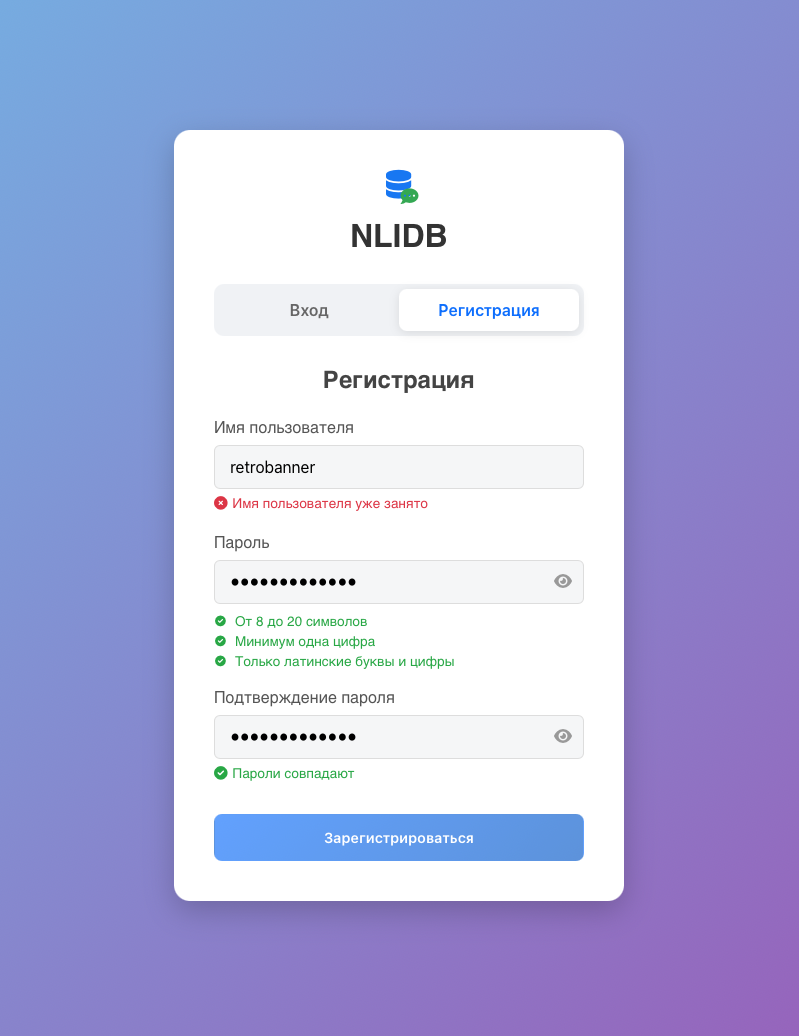
\includegraphics[width=\linewidth]{GUI/registration.png}
            \caption{Экран регистрации}
            \label{fig:registration}
      \end{subfigure}
      \hfill
      \begin{subfigure}[b]{0.48\textwidth}
            \centering
            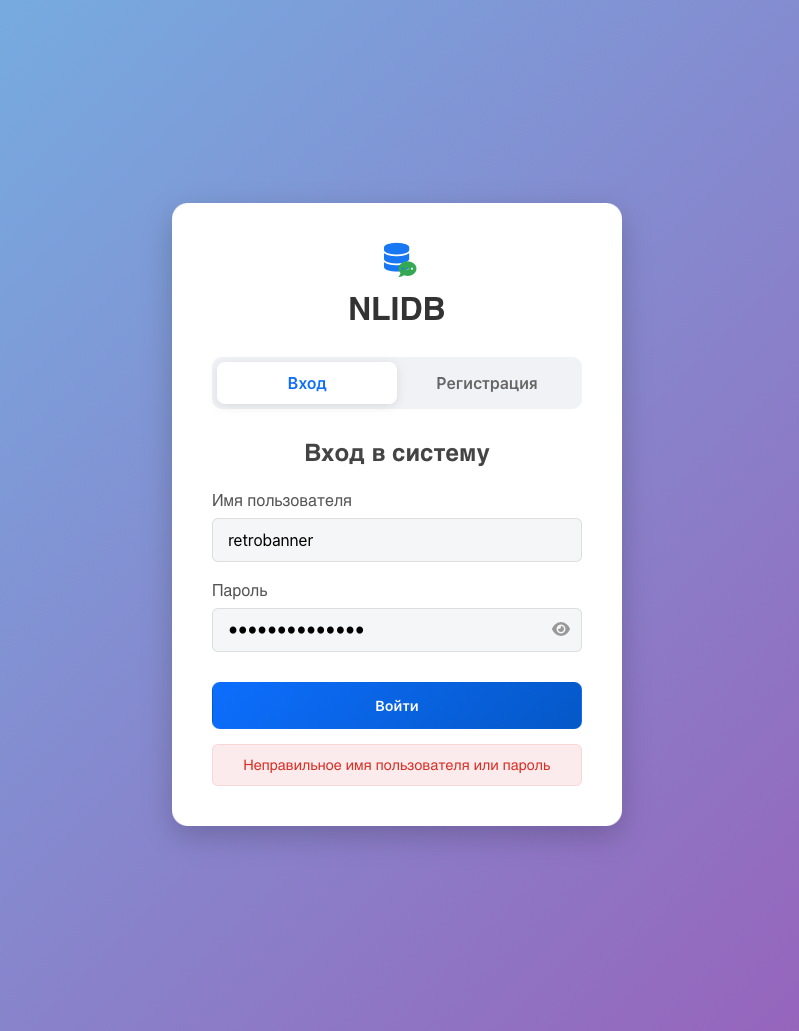
\includegraphics[width=\linewidth]{GUI/login.png}
            \caption{Экран входа в систему}
            \label{fig:login}
      \end{subfigure}
      \caption{Снимки экрана интерфейса аутентификации пользователя}
      \label{fig:auth_screens}
\end{figure}


\paragraph{Основной рабочий интерфейс}. После входа пользователь попадает на главный экран~---
«Конструктор запросов» (см.~рис.~\ref{fig:queries}). Это центральная рабочая область, разделенная на
две части. Слева расположена панель «Мои таблицы», где отображается список всех загруженных
пользователем таблиц. Кнопка «+» позволяет инициировать процесс добавления новой таблицы.

\begin{figure}[ht]
      \centering
      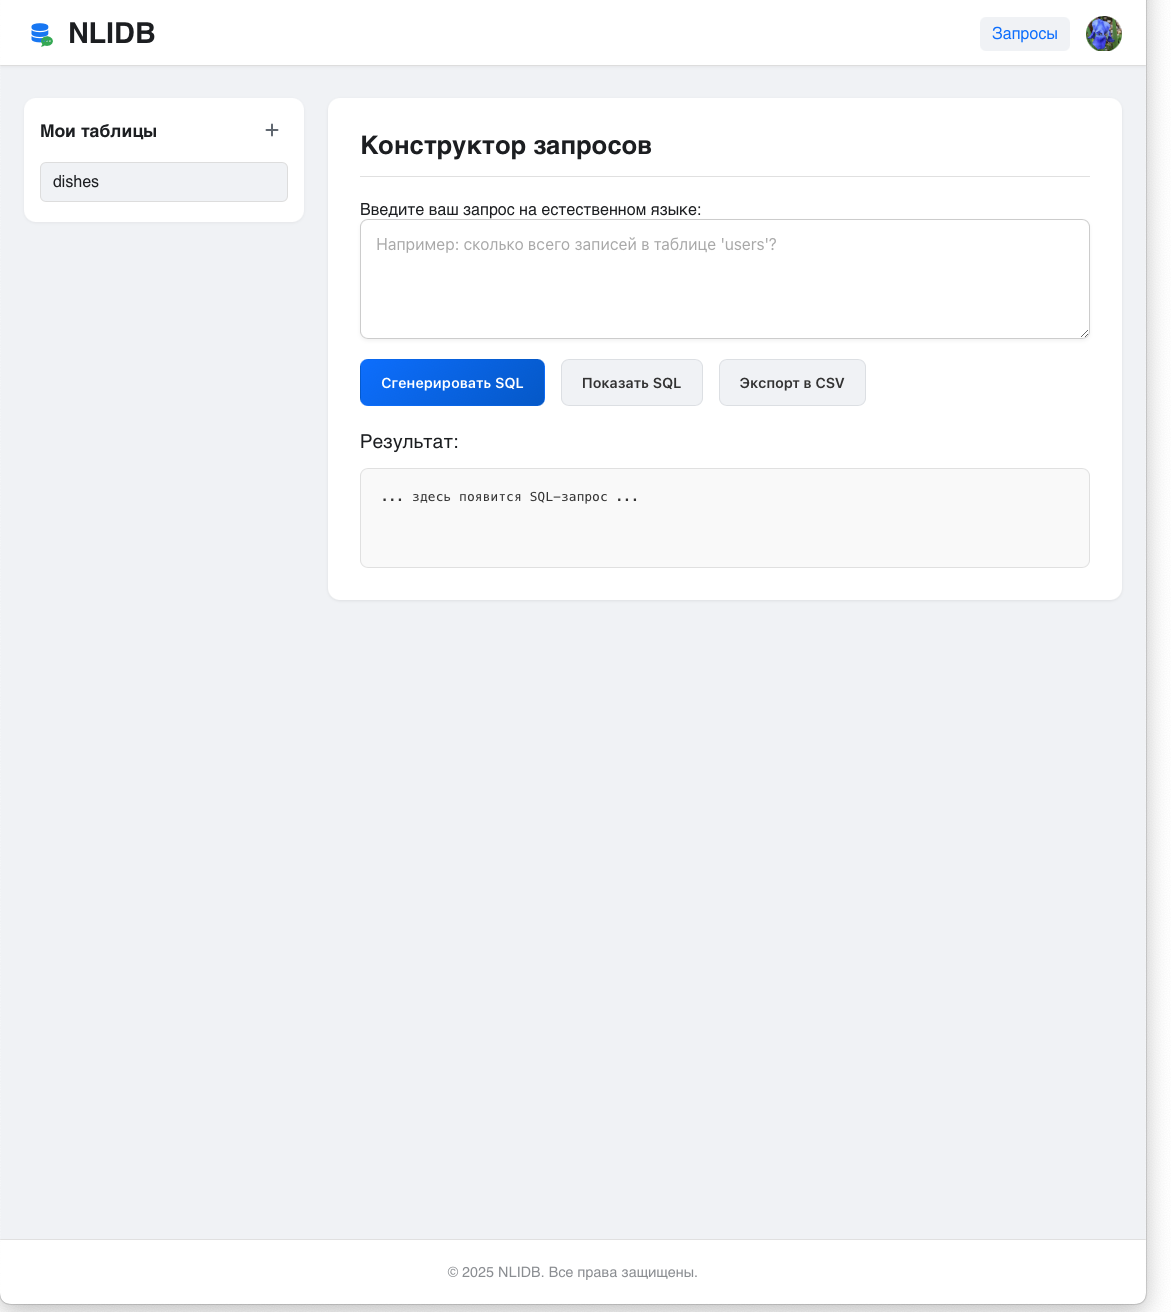
\includegraphics[width=\textwidth]{GUI/queries.png}
      \caption{Основной интерфейс конструктора запросов}
      \label{fig:queries}
\end{figure}

При нажатии на кнопку добавления таблицы открывается модальное окно
(см.~рис.~\ref{fig:table-uploading}), через которое пользователь может загрузить файл в формате CSV
или Excel. После выбора файла система автоматически анализирует его и отображает предварительный
просмотр первых 10 строк, что позволяет пользователю убедиться в корректности данных перед их
окончательной загрузкой.

\begin{figure}[ht]
      \centering
      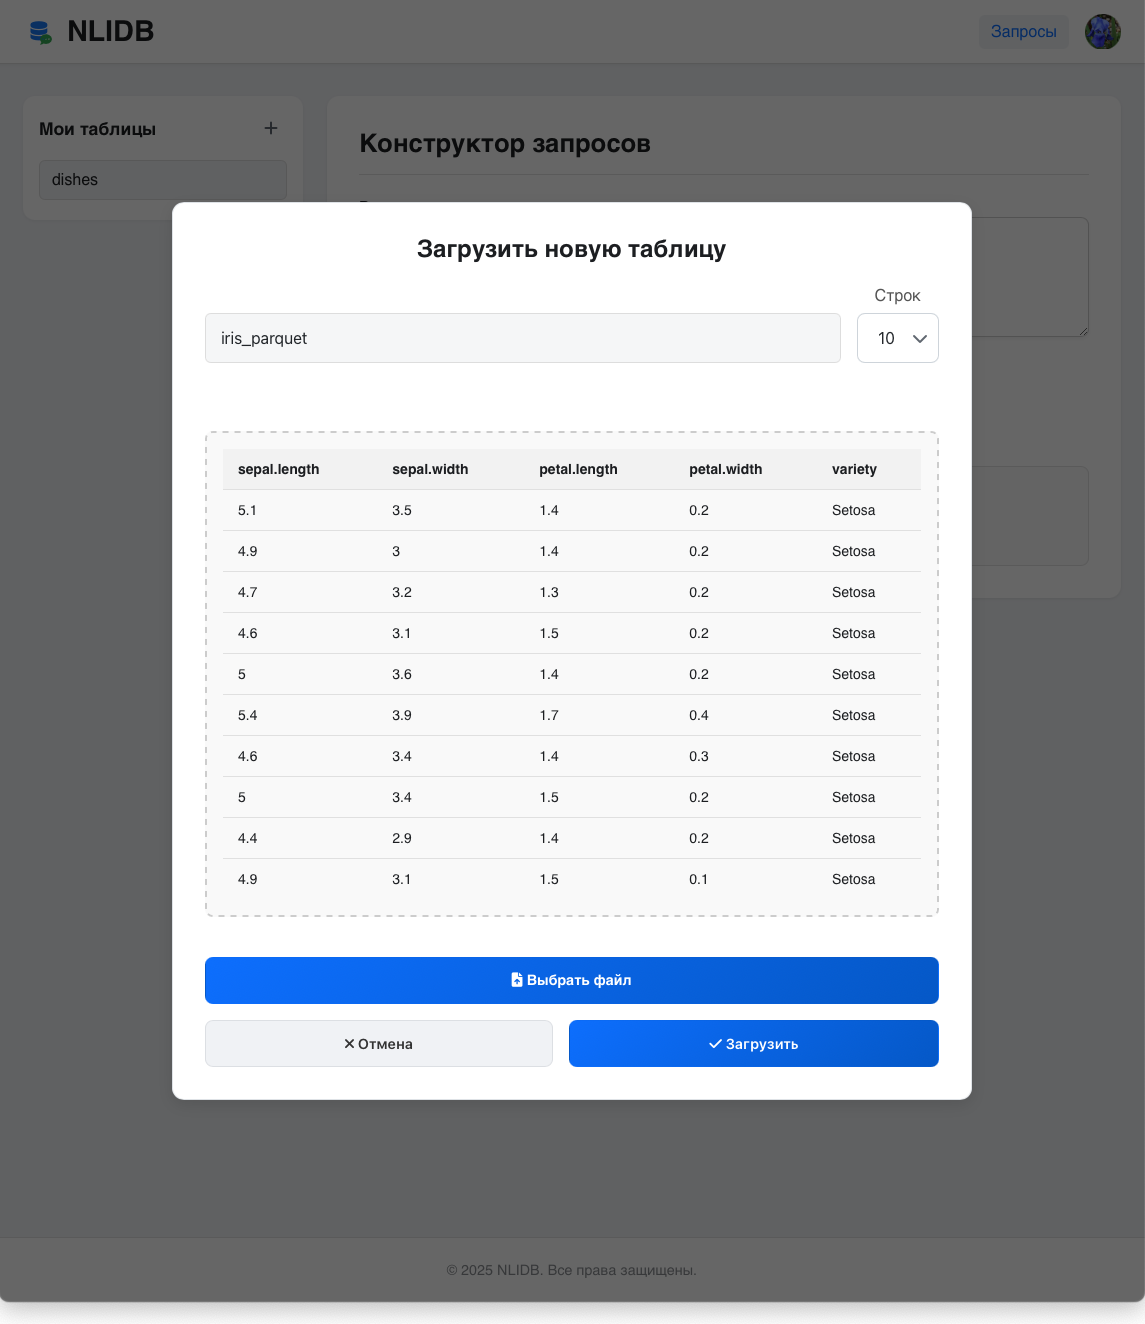
\includegraphics[width=\textwidth]{GUI/table-uploading.png}
      \caption{Модальное окно загрузки и предпросмотра новой таблицы}
      \label{fig:table-uploading}
\end{figure}

Основная часть экрана «Конструктор запросов» содержит большое текстовое поле для ввода запроса на
естественном языке. Ниже расположены кнопки для управления процессом: «Сгенерировать SQL», «Показать
SQL» и «Экспорт в CSV». В области «Результат» отображается таблица с данными, полученными после
выполнения запроса.

\paragraph{Настройки пользователя}. На странице настроек (см.~рис.~\ref{fig:settings}) пользователь
может управлять своим профилем.
Интерфейс разделен на три логических блока:
\begin{compactitem}
      \item \textbf{Смена аватара:} Пользователь может загрузить собственное изображение или удалить
      его, вернувшись к аватару по умолчанию, который генерируется автоматически. Модальное окно для
      смены аватара показано на рис.~\ref{fig:avatar-updating}.
      \item \textbf{Смена имени пользователя:} Поле для изменения псевдонима с мгновенной проверкой
      доступности нового имени.
      \item \textbf{Смена пароля:} Форма для безопасного обновления пароля с подтверждением старого и
      вводом нового пароля с соблюдением требований безопасности.
\end{compactitem}

\begin{figure}[ht]
      \centering
      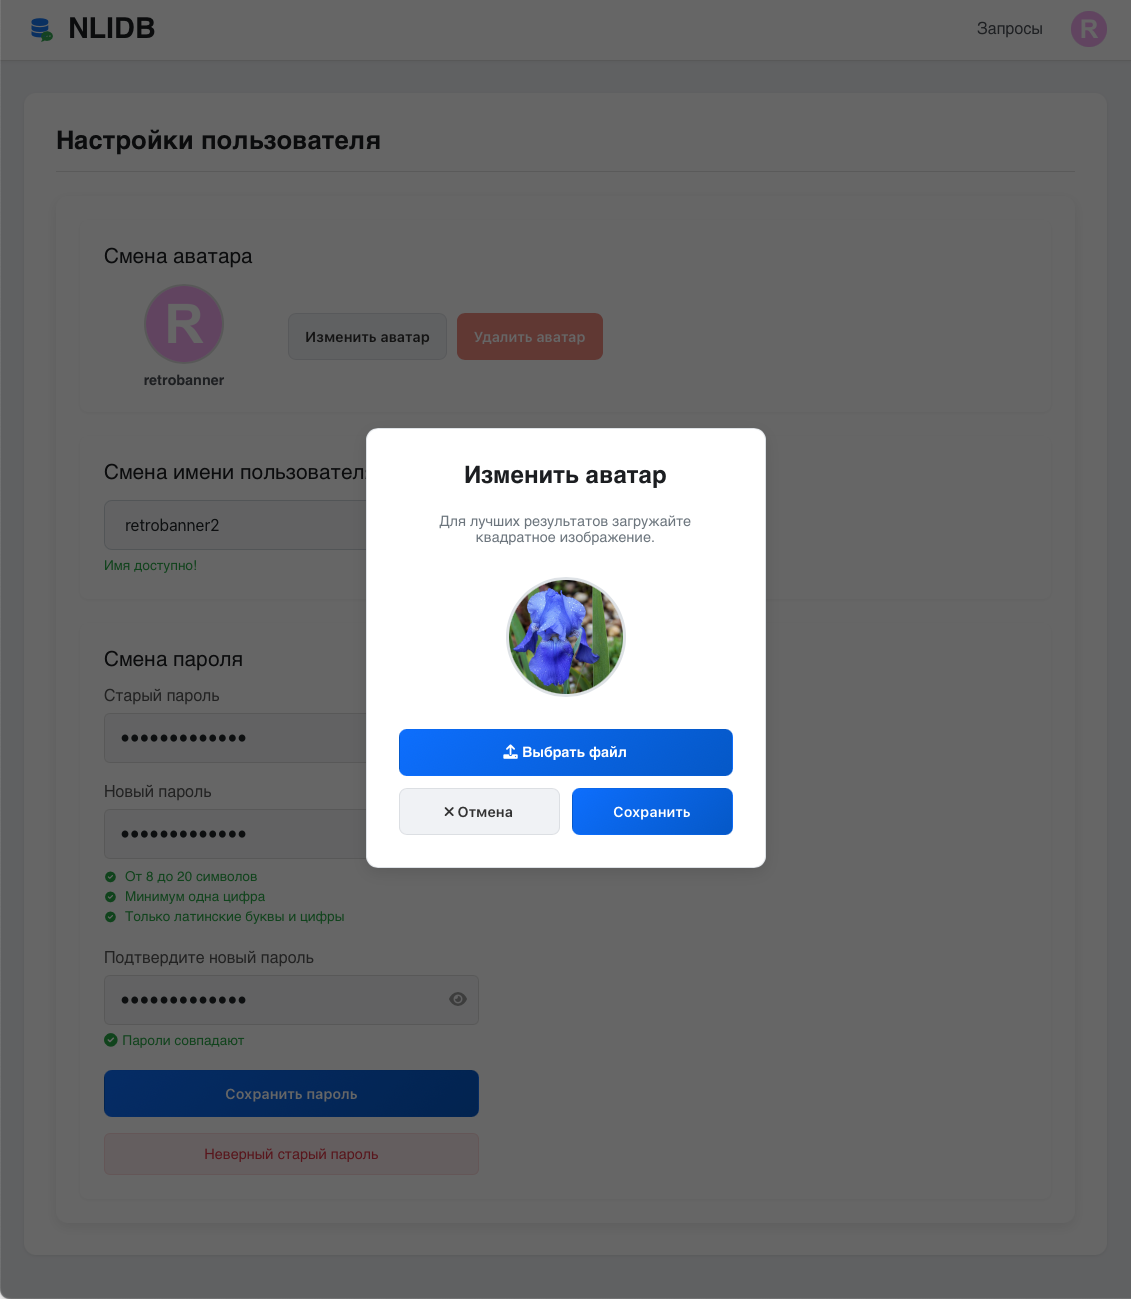
\includegraphics[width=0.8\textwidth]{GUI/avatar-updating.png}
      \caption{Модальное окно смены аватара}
      \label{fig:avatar-updating}
\end{figure}

\begin{figure}[ht]
      \centering
      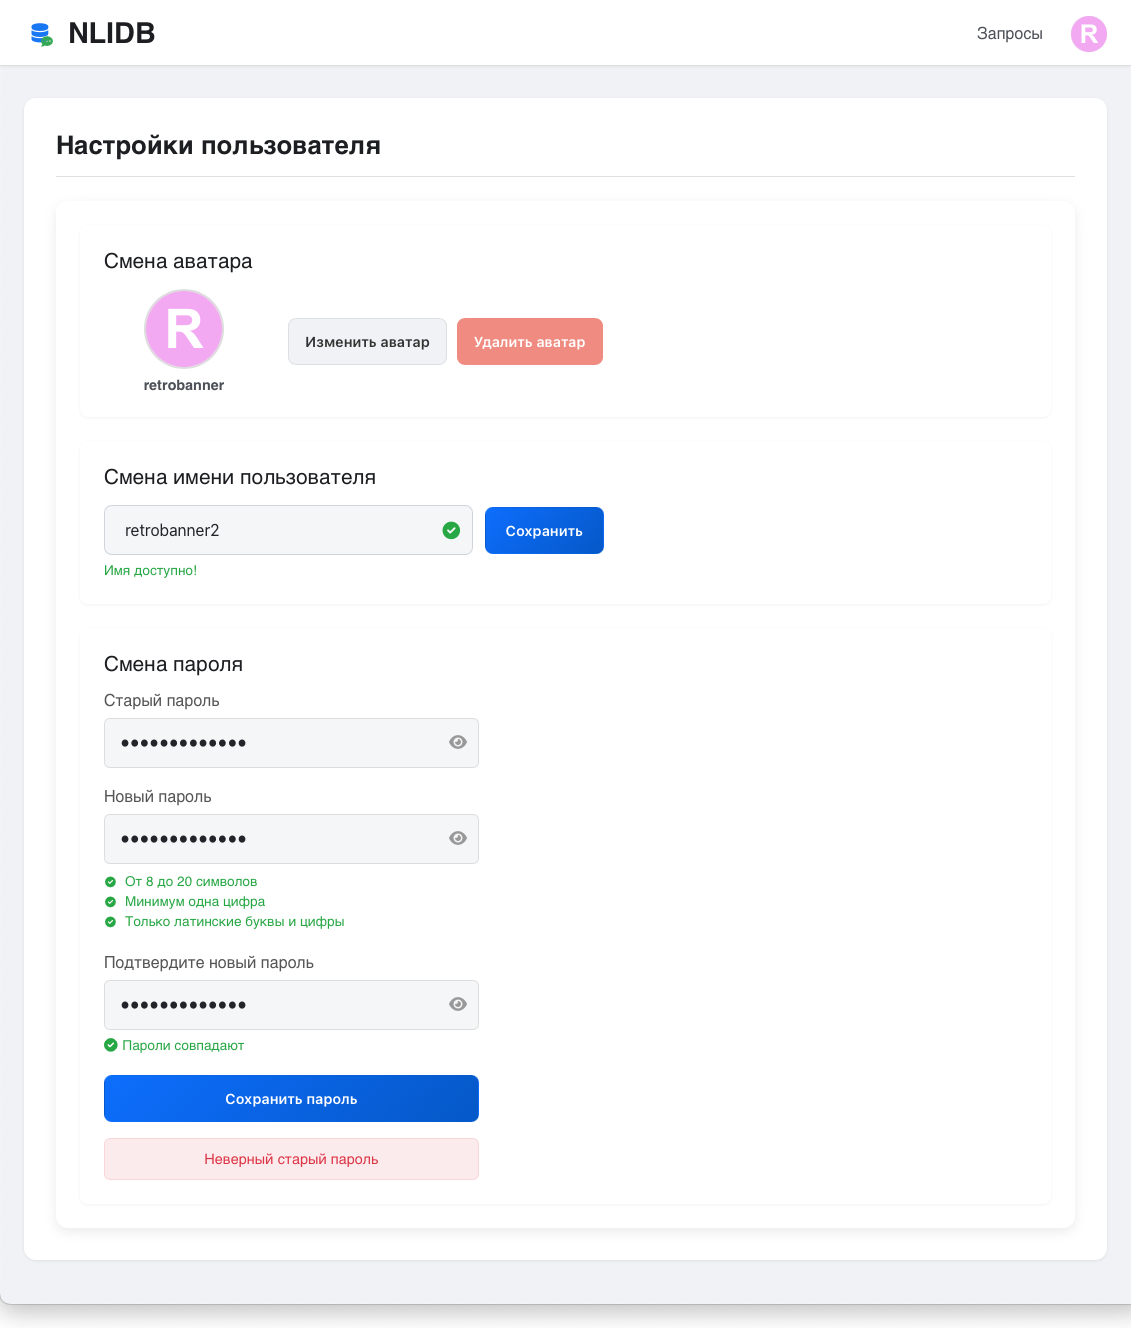
\includegraphics[width=0.8\textwidth]{GUI/settings.png}
      \caption{Страница настроек пользователя}
      \label{fig:settings}
\end{figure}

В целом, спроектированный графический интерфейс является логичным, неперегруженным и полностью
ориентированным на выполнение ключевых задач пользователя, что соответствует целям разработки данного
прототипа.




\section{Тестирование реализованного прототипа веб-сервиса}

Для проверки корректности работы, надежности и соответствия функциональным требованиям, изложенным в
предыдущих разделах, было проведено комплексное модульное тестирование разработанного прототипа.
Тестирование является неотъемлемым этапом жизненного цикла разработки, позволяющим выявить и устранить
потенциальные ошибки на ранней стадии и гарантировать стабильность системы.

\paragraph{Инструменты и среда тестирования}. В качестве основного фреймворка для написания и запуска
тестов был выбран \textbf{pytest}~--- современный и мощный инструмент для тестирования на Python. Для
взаимодействия с API-эндпоинтами приложения использовался \verb|TestClient| из состава фреймворка
FastAPI. Данный подход позволяет отправлять HTTP-запросы напрямую к приложению, не требуя запуска
реального веб-сервера, что значительно ускоряет выполнение тестов и упрощает их настройку.

Для обеспечения полной изоляции тестового окружения все тесты выполнялись на отдельной, временной базе
данных \textbf{SQLite}. Специальная фикстура в \verb|pytest| перед запуском каждого теста создавала
новую, чистую базу данных и удаляла ее после завершения. Это гарантирует, что тесты являются
независимыми друг от друга и результаты одного теста не влияют на последующие.

\paragraph{Структура и организация тестов}. Все автоматизированные тесты расположены в директории
\verb|/tests| и логически сгруппированы в модули, соответствующие структуре основного приложения
(\verb|test_users.py|, \verb|test_tables.py| и т.д.).

Ключевая логика подготовки тестового окружения вынесена в конфигурационный файл
\verb|tests/conftest.py|, где определены основные фикстуры:
\begin{compactitem}
      \item \verb|db|. Управляет жизненным циклом тестовой базы данных, обеспечивая ее создание и
      очистку.
      \item \verb|client|. Предоставляет экземпляр \verb|TestClient| для выполнения запросов от имени
      неаутентифицированного пользователя.
      \item \verb|authorized_client|. Ключевая фикстура для тестирования защищенных эндпоинтов. Она
      инкапсулирует логику создания временного пользователя через API, его последующей аутентификации
      и возвращает клиент с уже установленным токеном авторизации. Это позволяет значительно
      упростить код тестов для защищенных маршрутов.
\end{compactitem}

\paragraph{Тестовое покрытие}. Автоматизированные тесты охватывают все ключевые функциональные модули
разработанного прототипа:
\begin{compactitem}
      \item \textbf{Модуль аутентификации и управления пользователями:} Протестированы сценарии
      регистрации нового пользователя, входа в систему, получения и обновления данных профиля
      (включая смену пароля и аватара). Также покрыты случаи обработки ошибок, такие как попытка
      регистрации с уже существующим именем.
      \item \textbf{Модуль управления таблицами:} Протестированы все CRUD-операции
      (создание, чтение, обновление, удаление) для таблиц данных. Особое внимание уделено проверке
      прав доступа: тесты подтверждают, что пользователь не может получить доступ к таблицам,
      принадлежащим другому пользователю.
      \item \textbf{Внутренние сервисы:} Проведены тесты для отдельных сервисных функций в изоляции, в
      частности, для сервиса \verb|AvatarService|, отвечающего за генерацию аватаров по умолчанию.
\end{compactitem}

\paragraph{Результаты тестирования}. В общей сложности было разработано 47 автоматизированных тестов,
покрывающих описанный выше функционал. \textbf{Все 47 тестов успешно пройдены}, что подтверждается
выводом утилиты \verb|pytest| (см.~прил.~\ref{appendix-C}). В ходе выполнения тестов не было
зафиксировано никаких предупреждений (warnings).

Таким образом, комплексное тестирование подтверждает, что разработанный прототип веб-сервиса
функционирует корректно и в полном соответствии со спроектированной архитектурой и заявленными
функциональными требованиями.

\clearpage

\chapter*{Заключение}
\addcontentsline{toc}{chapter}{Заключение}

В заключении в тезисной форме необходимо отразить результаты работы:

\begin{itemize}
	\item аналитические (что изучено/проанализировано);
	\item теоретические;
	\item инженерные (что спроектировано);
	\item практические (что реализовано/внедрено).
\end{itemize}

Примерная формула такая: по каждому указанному пункту приводится по 3-5 результатов, каждый результат излагается в объеме до 5 фраз или предложений.

Также есть смысл привести предполагаемые направления для будущей работы.

Общий объем заключения не должен превышать 1,5 страниц (1 страницы для УИРов).


\setcounter{totalfigures}{\the\value{totalfigures}+\the\value{figure}}
\setcounter{figure}{0}
\setcounter{totaltables}{\the\value{totaltables}+\the\value{table}}
\setcounter{table}{0}
\setcounter{totallistings}{\the\value{totallistings}+\the\value{lstlisting}}
\setcounter{lstlisting}{0}

\makeatletter
\edef\@currentlabel{\the\value{totalfigures}}
\label{figures}
\edef\@currentlabel{\the\value{totaltables}}
\label{tables}
\edef\@currentlabel{\the\value{totallistings}}
\label{listings}
\makeatother

% --- СЕКЦИЯ БИБЛИОГРАФИИ ---

\clearpage

\phantomsection
\label{sec:bibliography}
\addcontentsline{toc}{chapter}{\bibname}	% Добавляем список литературы в оглавление
\printbibliography

\endrefsection

\label{end_of_main_text}

%--- КОНЕЦ СЕКЦИИ БИБЛИОГРАФИИ ---
%--- СЕКЦИЯ ПРИЛОЖЕНИЙ ---
\clearpage
\label{sec:appendices}

\begin{appendices}
    \chapter*{Приложения}
    \addcontentsline{toc}{chapter}{Приложения}

    % Изменяем поведение частей, разделов, подразделов для корректного попадания в TOC
    \let\oldchapter\chapter
    \renewcommand{\thechapter}{\Asbuk{chapter}}
    \renewcommand{\chapter}[1]{%
        \refstepcounter{chapter}%
        \oldchapter*{\appendixname~\thechapter.~#1}%
        \addcontentsline{toc}{section}{\appendixname~\thechapter.~#1}%
        \stepcounter{totalappendices}%
    }

    \let\oldsection\section
    \renewcommand{\section}[1]{
        \stepcounter{section}%
        \oldsection*{\thesection~#1}%
    }
    \let\oldsubsection\subsection
    \renewcommand{\subsection}[1]{
        \stepcounter{subsection}
        \oldsubsection*{\thesubsection~#1}
    }

    % Первое приложение не переносится на новую страницу
    \makeatletter
    \let\oldclearpage\clearpage
    \let\clearpage\relax
    \makeatother
    \chapter{Показатели XiYan-SQL в ключевых бенчмарках задачи Text-to-SQL}\label{appendix-A}

\begin{figure}[h]
	\centering
	\begin{subcaptiongroup}
		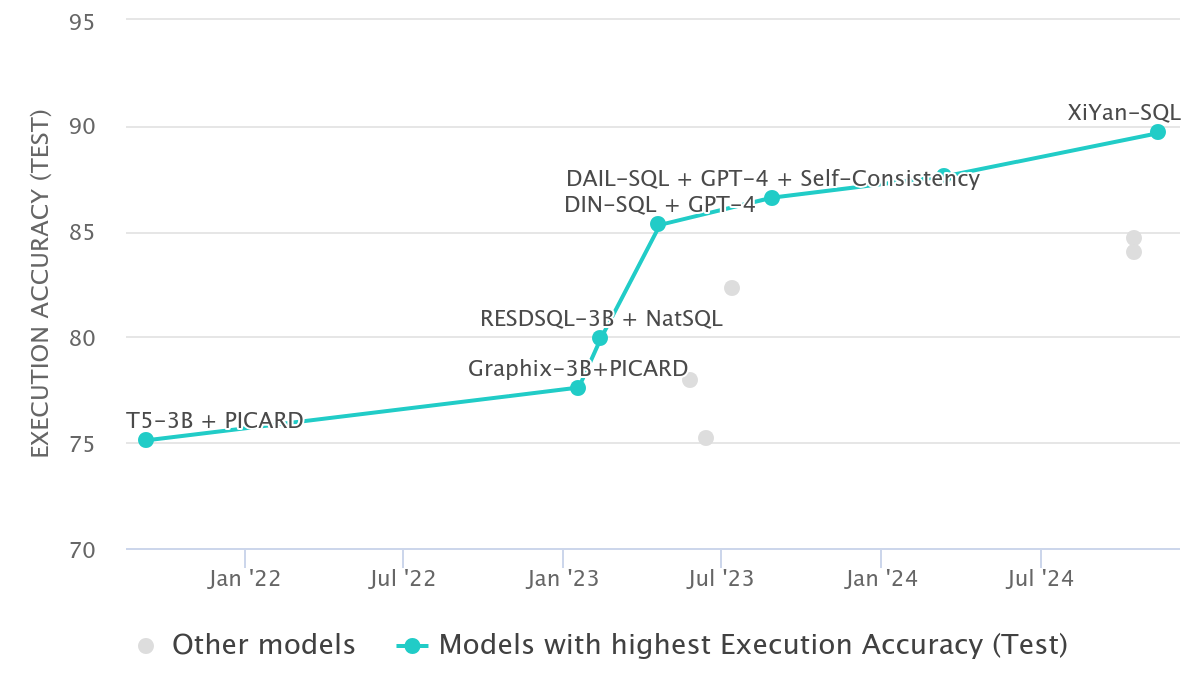
\includegraphics[width=0.85\textwidth]{literature-review/SOTA-Spider.png}
		\caption{Бенчмарк Spider}
		\label{fig:SOTA-Spider}
		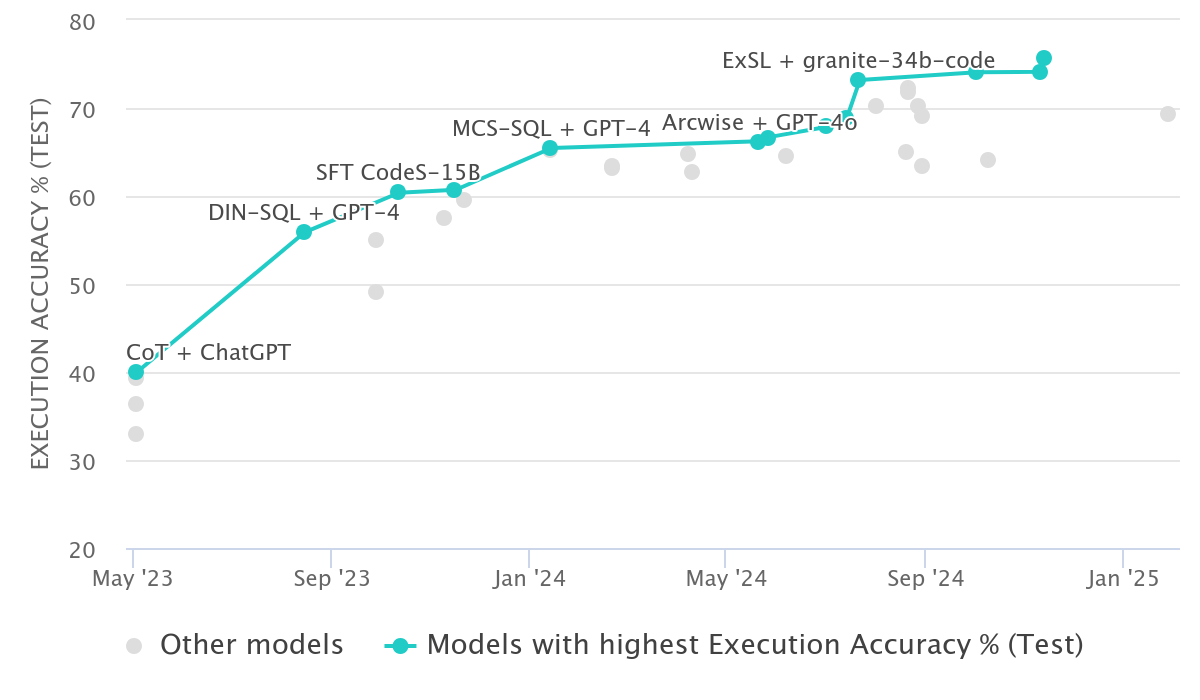
\includegraphics[width=0.85\textwidth]{literature-review/SOTA-BIRD.png}
		\caption{Бенчмарк BIRD}
		\label{fig:SOTA-Bird}
	\end{subcaptiongroup}
	\captionsetup{subrefformat=parens}
	\caption{Графики лидеров на бенчмарках Spider и BIRD}
	\label{fig:SOTA-Spider-Bird}
\end{figure}

%Далее приложения начинаются с новых страниц
\makeatletter
\let\clearpage\oldclearpage
\makeatother

\clearpage

\chapter{Фрагменты программного кода}\label{appendix-B}

\lstinputlisting[
	language=Python,
	label=lst:main_app,
	frame=lines,
	breaklines=true,
	caption={Точка входа в приложение (\texttt{main.py})}
]{4-listings/main.py}

\lstinputlisting[
	language=Python,
	label=lst:user_register,
	float=tb,frame=lines,
	caption=Реализация эндпоинта регистрации пользователя (\texttt{features/users/api.py})
]{4-listings/user_register.py}

\lstinputlisting[
	language=Python,
	label=lst:table_upload,
	float=tb,frame=lines,
	caption=Реализация эндпоинта загрузки таблицы (\texttt{features/tables/api.py})
]{4-listings/table_upload.py}

\lstinputlisting[
	language=Python,
	label=lst:table_preview,
	float=tb,frame=lines,
	caption=Реализация сервисной функции для получения превью таблицы (\texttt{services/table\_service.py})
]{4-listings/table_preview.py}

\lstinputlisting[
	language=Python,
	label=lst:nli-core-mock,
	float=tb,frame=lines,
	caption=Реализация модуля-эмулятора ядра NLIDB (\texttt{services/text\_to\_sql\_service.py})
]{4-listings/nli_core_mock.py}

\clearpage

\chapter{Вывод терминала об отчете тестирования прототипа}\label{appendix-C}

\lstinputlisting[
	language=bash,
	label=lst:test_report,
	frame=lines,
	breaklines=true,
	caption={Вывод терминала при запуске тестирования прототипа (\texttt{test-report.sh})}
]{4-listings/test-report.sh}

    % Восстанавливаем все как было
    \let\chapter\oldchapter
    \let\section\oldsection
    \let\subsection\oldsubsection
\end{appendices}

%--- КОНЕЦ СЕКЦИИ ПРИЛОЖЕНИЙ ---

\label{end_of_document}


\end{document}

